%! Licence = CC BY-NC-SA 4.0

%! Author = gianfluetsch
%! Date = 22.01.2022
%! Project = icth_summary

%import template
%! Licence = CC BY-NC-SA 4.0

%! Author = mariuszindel
%! Date = 24. Jan 2021
%! Project = latex-test-template


\documentclass[a4paper, landscape, 10pt]{scrartcl}

% charset
\usepackage[T1]{fontenc}
\usepackage[utf8]{inputenc}

% use language german
\usepackage[ngerman]{babel}

% format page size
\usepackage{geometry}
\geometry{top=1.2cm,left=0.4cm,right=0.4cm}
\textheight = 558pt

% tabular
\usepackage{tabularx}

% math
\usepackage{amsmath}
\usepackage{amssymb}
\usepackage{amsfonts}
\usepackage{enumitem}

% graphic
\usepackage{graphicx}
\graphicspath{{img/}}

% colors
\usepackage[dvipsnames]{xcolor}

% multi columns
\usepackage{multicol}

% make items compact
\setlist{topsep=0pt, leftmargin=3mm, nolistsep}
\setlength{\parindent}{0cm}

% author and institute
\newcommand{\AUTHOR}{Gian Flütsch}
\newcommand{\INSTITUTE}{Hochschule für Technik Rapperswil}

% define header and footer
\usepackage{fancyhdr}
\pagestyle{fancy}

\fancyhead[RO]{\AUTHOR| \INSTITUTE}
\fancyhead[LO]{\TITLE}
\fancyfoot[RO]{\DELIVERYDATE}
\renewcommand\headrulewidth{0pt}
\renewcommand\footrulewidth{0pt}
\headsep = -2pt
\footskip = 0pt

% define color
\definecolor{sectionColor}{HTML}{052639}
\definecolor{subSectionColor}{HTML}{468189}
\definecolor{subSubSectionColor}{HTML}{8DB9B1}
\definecolor{codeBackground}{RGB}{245,245,245}
\definecolor{gray}{rgb}{0.5,0.5,0.5}
\definecolor{darkGreen}{RGB}{0,150,0}
\definecolor{DarkPurple}{rgb}{0.4, 0.1, 0.4}
\definecolor{examcolor}{RGB}{255,0,0}

% define section format
\usepackage{sectsty}
\usepackage{titlesec}

\titleformat{name=\section}[block]{\sffamily\small}{}{0pt}{\colorsection}
\titlespacing*{\section}{0pt}{0pt}{0pt}
\newcommand{\colorsection}[1]{%
    \colorbox{sectionColor!80}{\parbox{0.98\linewidth}{\vspace{-1pt}\color{white}\ #1 \vspace{-2pt}}}}

% define subsection format
\titleformat{name=\subsection}[block]{\sffamily\small}{}{0pt}{\colorsubsection}
\titlespacing*{\subsection}{0pt}{0pt}{0pt}
\newcommand{\colorsubsection}[1]{%
    \colorbox{subSectionColor!80}{\parbox{0.98\linewidth}{\vspace{-1pt}\color{black}\ #1 \vspace{-2pt}}}}

% define subsubsection format
\titleformat{name=\subsubsection}[block]{\sffamily\small}{}{0pt}{\colorsubsubsection}
\titlespacing*{\subsubsection}{0pt}{0pt}{0pt}
\newcommand{\colorsubsubsection}[1]{%
    \colorbox{subSubSectionColor!60}{\parbox{0.98\linewidth}{\vspace{-1pt}\color{black}\ #1 \vspace{-2pt}}}}

% Define Subparagraph Format
\titleformat{name=\subparagraph}[block]{\sffamily\small}{}{0pt}{\colorparagraph}
\titlespacing*{\subparagraph}{0pt}{0pt}{0pt}
\newcommand{\colorparagraph}[1]{%
    \colorbox{examcolor!80}{\parbox{0.98\linewidth}{\vspace{-1pt}\color{black}\ Lab: #1 \vspace{-2pt}}}}


% import code listings
\usepackage{listings}
\usepackage{beramono}
%! Licence = CC BY-NC-SA 4.0

%! Author = gianfluetsch
%! Date = 07.09.2021
%! Project = Latex-documentation-template

\lstdefinestyle{Java}{
    language=java,
    backgroundcolor = \color{codeBackground},       %color for the background
    basicstyle=\ttfamily\scriptsize,                % font size/family/etc. for source
    keywordstyle=\color{RoyalBlue}\ttfamily,        % style of keywords in source language
    stringstyle=\color{darkGreen}\ttfamily,         % style of strings in source language
    commentstyle=\color{DarkPurple!60}\ttfamily,    % style of comments in source language
    escapeinside={£}{£},                            % specify characters to escape from source code to LATEX
    showspaces=false,                               % emphasize spaces in code (true/false)
    showstringspaces=false,
    showtabs=false,                                 % emphasize tabulators in code (true/false)
    numbers=left,                                   % position of line numbers (left/right/none)
    numberstyle=\tiny\color{darkgray}\ttfamily,     % style used for line-numbers
    stepnumber=1,                                   % distance of line-numbers from the code
    tabsize=1,                                      % default tabsize
    breaklines=true,                                % automatic line-breaking
    breakatwhitespace=true,                         % sets if automatic breaks should only happen at whitespaces
    frame=single,                                   % showing frame outside code (none/leftline/topline/bottomline/lines/single/shadowbox)
    xleftmargin=15pt,
    xrightmargin=15pt,
    frameround=tttt,                            % enable round corners
    rulecolor = \color{lightgray},              % Specify the colour of the frame-box
    aboveskip = 6pt,
    belowskip = 15pt,
    captionpos = b                              % position of caption (t/b)
}

\lstdefinestyle{CSharp}{
    language=[Sharp]C,
    backgroundcolor = \color{codeBackground},       %color for the background
    basicstyle=\ttfamily\scriptsize,                % font size/family/etc. for source
    keywordstyle=\color{RoyalBlue}\ttfamily,        % style of keywords in source language
    stringstyle=\color{darkGreen}\ttfamily,         % style of strings in source language
    commentstyle=\color{DarkPurple!60}\ttfamily,    % style of comments in source language
    escapeinside={£}{£},                            % specify characters to escape from source code to LATEX
    showspaces=false,                               % emphasize spaces in code (true/false)
    showstringspaces=false,
    showtabs=false,                                 % emphasize tabulators in code (true/false)
    numbers=left,                                   % position of line numbers (left/right/none)
    numberstyle=\tiny\color{darkgray}\ttfamily,     % style used for line-numbers
    stepnumber=1,                                   % distance of line-numbers from the code
    tabsize=1,                                      % default tabsize
    breaklines=true,                                % automatic line-breaking
    breakatwhitespace=true,                         % sets if automatic breaks should only happen at whitespaces
    frame=single,                                   % showing frame outside code (none/leftline/topline/bottomline/lines/single/shadowbox)
    xleftmargin=15pt,
    xrightmargin=15pt,
    frameround=tttt,                            % enable round corners
    rulecolor = \color{lightgray},              % Specify the colour of the frame-box
    aboveskip = 6pt,
    belowskip = 15pt,
    captionpos = b                              % position of caption (t/b)
}

\lstdefinestyle{JavaScript}{
    keywords={typeof, new, true, false, catch, function, return, null, catch, switch, var, if, in, while, do, else, case, break},
    ndkeywords={class, export, boolean, throw, implements, import, this},
    comment=[l]{//},
    backgroundcolor = \color{codeBackground},       %color for the background
    basicstyle=\ttfamily\scriptsize,                % font size/family/etc. for source
    keywordstyle=\color{RoyalBlue}\ttfamily,        % style of keywords in source language
    stringstyle=\color{darkGreen}\ttfamily,         % style of strings in source language
    commentstyle=\color{DarkPurple!60}\ttfamily,    % style of comments in source language
    escapeinside={£}{£},                            % specify characters to escape from source code to LATEX
    showspaces=false,                               % emphasize spaces in code (true/false)
    showstringspaces=false,
    showtabs=false,                                 % emphasize tabulators in code (true/false)
    numbers=left,                                   % position of line numbers (left/right/none)
    numberstyle=\tiny\color{darkgray}\ttfamily,     % style used for line-numbers
    stepnumber=1,                                   % distance of line-numbers from the code
    tabsize=1,                                      % default tabsize
    breaklines=true,                                % automatic line-breaking
    breakatwhitespace=true,                         % sets if automatic breaks should only happen at whitespaces
    frame=single,                                   % showing frame outside code (none/leftline/topline/bottomline/lines/single/shadowbox)
    xleftmargin=15pt,
    xrightmargin=15pt,
    frameround=tttt,                            % enable round corners
    rulecolor = \color{lightgray},              % Specify the colour of the frame-box
    aboveskip = 6pt,
    belowskip = 15pt,
    captionpos = b                              % position of caption (t/b)
}

\lstdefinestyle{HTML}{
    language=HTML,
    backgroundcolor = \color{codeBackground},       %color for the background
    basicstyle=\ttfamily\scriptsize,                % font size/family/etc. for source
    keywordstyle=\color{RoyalBlue}\ttfamily,        % style of keywords in source language
    stringstyle=\color{darkGreen}\ttfamily,         % style of strings in source language
    commentstyle=\color{DarkPurple!60}\ttfamily,    % style of comments in source language
    escapeinside={£}{£},                            % specify characters to escape from source code to LATEX
    showspaces=false,                               % emphasize spaces in code (true/false)
    showstringspaces=false,
    showtabs=false,                                 % emphasize tabulators in code (true/false)
    numbers=left,                                   % position of line numbers (left/right/none)
    numberstyle=\tiny\color{darkgray}\ttfamily,     % style used for line-numbers
    stepnumber=1,                                   % distance of line-numbers from the code
    tabsize=1,                                      % default tabsize
    breaklines=true,                                % automatic line-breaking
    breakatwhitespace=true,                         % sets if automatic breaks should only happen at whitespaces
    frame=single,                                   % showing frame outside code (none/leftline/topline/bottomline/lines/single/shadowbox)
    xleftmargin=15pt,
    xrightmargin=15pt,
    frameround=tttt,                            % enable round corners
    rulecolor = \color{lightgray},              % Specify the colour of the frame-box
    aboveskip = 6pt,
    belowskip = 15pt,
    captionpos = b                              % position of caption (t/b)
}

\lstdefinestyle{Python}{
    language=Python,
    backgroundcolor = \color{codeBackground},       %color for the background
    basicstyle=\ttfamily\scriptsize,                % font size/family/etc. for source
    keywordstyle=\color{RoyalBlue}\ttfamily,        % style of keywords in source language
    stringstyle=\color{darkGreen}\ttfamily,         % style of strings in source language
    commentstyle=\color{DarkPurple!60}\ttfamily,    % style of comments in source language
    escapeinside={£}{£},                            % specify characters to escape from source code to LATEX
    showspaces=false,                               % emphasize spaces in code (true/false)
    showstringspaces=false,
    showtabs=false,                                 % emphasize tabulators in code (true/false)
    numbers=left,                                   % position of line numbers (left/right/none)
    numberstyle=\tiny\color{darkgray}\ttfamily,     % style used for line-numbers
    stepnumber=1,                                   % distance of line-numbers from the code
    tabsize=1,                                      % default tabsize
    breaklines=true,                                % automatic line-breaking
    breakatwhitespace=true,                         % sets if automatic breaks should only happen at whitespaces
    frame=single,                                   % showing frame outside code (none/leftline/topline/bottomline/lines/single/shadowbox)
    xleftmargin=15pt,
    xrightmargin=15pt,
    frameround=tttt,                            % enable round corners
    rulecolor = \color{lightgray},              % Specify the colour of the frame-box
    aboveskip = 6pt,
    belowskip = 15pt,
    captionpos = b                              % position of caption (t/b)
}

\lstdefinestyle{bash}{
    language=bash,
    backgroundcolor = \color{codeBackground},       %color for the background
    basicstyle=\ttfamily\scriptsize,                % font size/family/etc. for source
    keywordstyle=\color{RoyalBlue}\ttfamily,        % style of keywords in source language
    stringstyle=\color{darkGreen}\ttfamily,         % style of strings in source language
    commentstyle=\color{DarkPurple!60}\ttfamily,    % style of comments in source language
    escapeinside={£}{£},                            % specify characters to escape from source code to LATEX
    showspaces=false,                               % emphasize spaces in code (true/false)
    showstringspaces=false,
    showtabs=false,                                 % emphasize tabulators in code (true/false)
    numbers=left,                                   % position of line numbers (left/right/none)
    numberstyle=\tiny\color{darkgray}\ttfamily,     % style used for line-numbers
    stepnumber=1,                                   % distance of line-numbers from the code
    tabsize=1,                                      % default tabsize
    breaklines=true,                                % automatic line-breaking
    breakatwhitespace=true,                         % sets if automatic breaks should only happen at whitespaces
    frame=single,                                   % showing frame outside code (none/leftline/topline/bottomline/lines/single/shadowbox)
    xleftmargin=15pt,
    xrightmargin=15pt,
    frameround=tttt,                            % enable round corners
    rulecolor = \color{lightgray},              % Specify the colour of the frame-box
    aboveskip = 6pt,
    belowskip = 15pt,
    captionpos = b                              % position of caption (t/b)
}

\lstdefinestyle{LaTeX}{
    language=TeX,
    backgroundcolor = \color{codeBackground},       %color for the background
    basicstyle=\ttfamily\scriptsize,                % font size/family/etc. for source
    keywordstyle=\color{RoyalBlue}\ttfamily,        % style of keywords in source language
    stringstyle=\color{darkGreen}\ttfamily,         % style of strings in source language
    commentstyle=\color{DarkPurple!60}\ttfamily,    % style of comments in source language
    escapeinside={£}{£},                            % specify characters to escape from source code to LATEX
    showspaces=false,                               % emphasize spaces in code (true/false)
    showstringspaces=false,
    showtabs=false,                                 % emphasize tabulators in code (true/false)
    numbers=left,                                   % position of line numbers (left/right/none)
    numberstyle=\tiny\color{darkgray}\ttfamily,     % style used for line-numbers
    stepnumber=1,                                   % distance of line-numbers from the code
    tabsize=1,                                      % default tabsize
    breaklines=true,                                % automatic line-breaking
    breakatwhitespace=true,                         % sets if automatic breaks should only happen at whitespaces
    frame=single,                                   % showing frame outside code (none/leftline/topline/bottomline/lines/single/shadowbox)
    xleftmargin=15pt,
    xrightmargin=15pt,
    frameround=tttt,                            % enable round corners
    rulecolor = \color{lightgray},              % Specify the colour of the frame-box
    aboveskip = 6pt,
    belowskip = 15pt,
    captionpos = b                              % position of caption (t/b)
}

\lstdefinelanguage{XML}
{
	backgroundcolor = \color{codeBackground},
	basicstyle=\ttfamily\scriptsize,
	morestring=[b]",
	moredelim=[s][\bfseries\color{black}]{>}{<},
	moredelim=[s][\bfseries\color{black}]{</}{>},
	% moredelim=[l][\bfseries\color{black}]{/>},
	% moredelim=[l][\bfseries\color{black}]{>},
	morecomment=[s]{<?}{?>},
	morecomment=[s]{<!--}{-->},
	commentstyle=\color{darkGreen},
	stringstyle=\color{blue},
	identifierstyle=\color{red},
	frame=single,                                   % showing frame outside code (none/leftline/topline/bottomline/lines/single/shadowbox)
    xleftmargin=15pt,
    xrightmargin=15pt,
    frameround=tttt,  
}

\lstdefinelanguage{PowerShell}{
	morekeywords={
		Add-Content,Add-PSSnapin,Clear-Content,Clear-History,Clear-Host,Clear-Item,Clear-ItemProperty,Clear-Variable,Compare-Object,Connect-PSSession,ConvertFrom-String,Convert-Path,Copy-Item,Copy-ItemProperty,Disable-PSBreakpoint,Disconnect-PSSession,Enable-PSBreakpoint,Enter-PSSession,Exit-PSSession,Export-Alias,Export-Csv,Export-PSSession,ForEach-Object,Format-Custom,Format-Hex,Format-List,Format-Table,Format-Wide,Get-Alias,Get-ChildItem,Get-Clipboard,Get-Command,Get-ComputerInfo,Get-Content,Get-History,Get-Item,Get-ItemProperty,Get-ItemPropertyValue,Get-Job,Get-Location,Get-Member,Get-Module,Get-Process,Get-PSBreakpoint,Get-PSCallStack,Get-PSDrive,Get-PSSession,Get-PSSnapin,Get-Service,Get-TimeZone,Get-Unique,Get-Variable,Get-WmiObject,Group-Object,help,Import-Alias,Import-Csv,Import-Module,Import-PSSession,Invoke-Command,Invoke-Expression,Invoke-History,Invoke-Item,Invoke-RestMethod,Invoke-WebRequest,Invoke-WmiMethod,Measure-Object,mkdir,Move-Item,Move-ItemProperty,New-Alias,New-Item,New-Module,New-PSDrive,New-PSSession,New-PSSessionConfigurationFile,New-Variable,Out-GridView,Out-Host,Out-Printer,Pop-Location,powershell_ise.exe,Push-Location,Receive-Job,Receive-PSSession,Remove-Item,Remove-ItemProperty,Remove-Job,Remove-Module,Remove-PSBreakpoint,Remove-PSDrive,Remove-PSSession,Remove-PSSnapin,Remove-Variable,Remove-WmiObject,Rename-Item,Rename-ItemProperty,Resolve-Path,Resume-Job,Select-Object,Select-String,Set-Alias,Set-Clipboard,Set-Content,Set-Item,Set-ItemProperty,Set-Location,Set-PSBreakpoint,Set-TimeZone,Set-Variable,Set-WmiInstance,Show-Command,Sort-Object,Start-Job,Start-Process,Start-Service,Start-Sleep,Stop-Job,Stop-Process,Stop-Service,Suspend-Job,Tee-Object,Trace-Command,Wait-Job,Where-Object,Write-Output
	},
	morekeywords={
		Add-AppxPackage,Add-AppxProvisionedPackage,Add-AppxVolume,Add-BitsFile,Add-CertificateEnrollmentPolicyServer,Add-Computer,Add-Content,Add-History,Add-JobTrigger,Add-KdsRootKey,Add-LocalGroupMember,Add-Member,Add-PSSnapin,Add-Type,Add-WindowsCapability,Add-WindowsDriver,Add-WindowsImage,Add-WindowsPackage,Checkpoint-Computer,Clear-Content,Clear-EventLog,Clear-History,Clear-Item,Clear-ItemProperty,Clear-KdsCache,Clear-RecycleBin,Clear-Tpm,Clear-Variable,Clear-WindowsCorruptMountPoint,Compare-Object,Complete-BitsTransfer,Complete-DtiagnosticTransaction,Complete-Transaction,Confirm-SecureBootUEFI,Connect-PSSession,Connect-WSMan,ConvertFrom-Csv,ConvertFrom-Json,ConvertFrom-SecureString,ConvertFrom-String,ConvertFrom-StringData,Convert-Path,Convert-String,ConvertTo-Csv,ConvertTo-Html,ConvertTo-Json,ConvertTo-ProcessMitigationPolicy,ConvertTo-SecureString,ConvertTo-TpmOwnerAuth,ConvertTo-Xml,Copy-Item,Copy-ItemProperty,Debug-Job,Debug-Process,Debug-Runspace,Disable-AppBackgroundTaskDiagnosticLog,Disable-ComputerRestore,Disable-JobTrigger,Disable-LocalUser,Disable-PSBreakpoint,Disable-PSRemoting,Disable-PSSessionConfiguration,Disable-RunspaceDebug,Disable-ScheduledJob,Disable-TlsCipherSuite,Disable-TlsEccCurve,Disable-TlsSessionTicketKey,Disable-TpmAutoProvisioning,Disable-WindowsErrorReporting,Disable-WindowsOptionalFeature,Disable-WSManCredSSP,Disconnect-PSSession,Disconnect-WSMan,Dismount-AppxVolume,Dismount-WindowsImage,Enable-AppBackgroundTaskDiagnosticLog,Enable-ComputerRestore,Enable-JobTrigger,Enable-LocalUser,Enable-PSBreakpoint,Enable-PSRemoting,Enable-PSSessionConfiguration,Enable-RunspaceDebug,Enable-ScheduledJob,Enable-TlsCipherSuite,Enable-TlsEccCurve,Enable-TlsSessionTicketKey,Enable-TpmAutoProvisioning,Enable-WindowsErrorReporting,Enable-WindowsOptionalFeature,Enable-WSManCredSSP,Enter-PSHostProcess,Enter-PSSession,Exit-PSHostProcess,Exit-PSSession,Expand-WindowsCustomDataImage,Expand-WindowsImage,Export-Alias,Export-BinaryMiLog,Export-Certificate,Export-Clixml,Export-Console,Export-Counter,Export-Csv,Export-FormatData,Export-ModuleMember,Export-PfxCertificate,Export-ProvisioningPackage,Export-PSSession,Export-StartLayout,Export-StartLayoutEdgeAssets,Export-TlsSessionTicketKey,Export-Trace,Export-WindowsCapabilitySource,Export-WindowsDriver,Export-WindowsImage,Find-Package,Find-PackageProvider,ForEach-Object,Format-Custom,Format-List,Format-SecureBootUEFI,Format-Table,Format-Wide,Get-Acl,Get-Alias,Get-AppxDefaultVolume,Get-AppxPackage,Get-AppxPackageManifest,Get-AppxProvisionedPackage,Get-AppxVolume,Get-AuthenticodeSignature,Get-BitsTransfer,Get-Certificate,Get-CertificateAutoEnrollmentPolicy,Get-CertificateEnrollmentPolicyServer,Get-CertificateNotificationTask,Get-ChildItem,Get-CimAssociatedInstance,Get-CimClass,Get-CimInstance,Get-CimSession,Get-Clipboard,Get-CmsMessage,Get-Command,Get-ComputerInfo,Get-ComputerRestorePoint,Get-Content,Get-ControlPanelItem,Get-Counter,Get-Credential,Get-Culture,Get-DAPolicyChange,Get-Date,Get-DeliveryOptimizationLog,Get-DeliveryOptimizationPerfSnap,Get-DeliveryOptimizationPerfSnapThisMonth,Get-DeliveryOptimizationStatus,Get-DODownloadMode,Get-DOPercentageMaxBackgroundBandwidth,Get-DOPercentageMaxForegroundBandwidth,Get-Event,Get-EventLog,Get-EventSubscriber,Get-ExecutionPolicy,Get-FormatData,Get-Help,Get-History,Get-Host,Get-HotFix,Get-Item,Get-ItemProperty,Get-ItemPropertyValue,Get-Job,Get-JobTrigger,Get-KdsConfiguration,Get-KdsRootKey,Get-LocalGroup,Get-LocalGroupMember,Get-LocalUser,Get-Location,Get-Member,Get-Module,Get-Package,Get-PackageProvider,Get-PackageSource,Get-PfxCertificate,Get-PfxData,Get-PmemDisk,Get-PmemPhysicalDevice,Get-PmemUnusedRegion,Get-Process,Get-ProcessMitigation,Get-ProvisioningPackage,Get-PSBreakpoint,Get-PSCallStack,Get-PSDrive,Get-PSHostProcessInfo,Get-PSProvider,Get-PSReadlineKeyHandler,Get-PSReadlineOption,Get-PSSession,Get-PSSessionCapability,Get-PSSessionConfiguration,Get-PSSnapin,Get-Random,Get-Runspace,Get-RunspaceDebug,Get-ScheduledJob,Get-ScheduledJobOption,Get-SecureBootPolicy,Get-SecureBootUEFI,Get-Service,Get-TimeZone,Get-TlsCipherSuite,Get-TlsEccCurve,Get-Tpm,Get-TpmEndorsementKeyInfo,Get-TpmSupportedFeature,Get-TraceSource,Get-Transaction,Get-TroubleshootingPack,Get-TrustedProvisioningCertificate,Get-TypeData,Get-UICulture,Get-Unique,Get-Variable,Get-WIMBootEntry,Get-WinAcceptLanguageFromLanguageListOptOut,Get-WinCultureFromLanguageListOptOut,Get-WinDefaultInputMethodOverride,Get-WindowsCapability,Get-WindowsDeveloperLicense,Get-WindowsDriver,Get-WindowsEdition,Get-WindowsErrorReporting,Get-WindowsImage,Get-WindowsImageContent,Get-WindowsOptionalFeature,Get-WindowsPackage,Get-WindowsSearchSetting,Get-WinEvent,Get-WinHomeLocation,Get-WinLanguageBarOption,Get-WinSystemLocale,Get-WinUILanguageOverride,Get-WinUserLanguageList,Get-WmiObject,Get-WSManCredSSP,Get-WSManInstance,Group-Object,Import-Alias,Import-BinaryMiLog,Import-Certificate,Import-Clixml,Import-Counter,Import-Csv,Import-LocalizedData,Import-Module,Import-PackageProvider,Import-PfxCertificate,Import-PSSession,Import-StartLayout,Import-TpmOwnerAuth,Initialize-PmemPhysicalDevice,Initialize-Tpm,Install-Package,Install-PackageProvider,Install-ProvisioningPackage,Install-TrustedProvisioningCertificate,Invoke-CimMethod,Invoke-Command,Invoke-CommandInDesktopPackage,Invoke-DscResource,Invoke-Expression,Invoke-History,Invoke-Item,Invoke-RestMethod,Invoke-TroubleshootingPack,Invoke-WebRequest,Invoke-WmiMethod,Invoke-WSManAction,Join-DtiagnosticResourceManager,Join-Path,Limit-EventLog,Measure-Command,Measure-Object,Mount-AppxVolume,Mount-WindowsImage,Move-AppxPackage,Move-Item,Move-ItemProperty,New-Alias,New-CertificateNotificationTask,New-CimInstance,New-CimSession,New-CimSessionOption,New-DtiagnosticTransaction,New-Event,New-EventLog,New-FileCatalog,New-Item,New-ItemProperty,New-JobTrigger,New-LocalGroup,New-LocalUser,New-Module,New-ModuleManifest,New-NetIPsecAuthProposal,New-NetIPsecMainModeCryptoProposal,New-NetIPsecQuickModeCryptoProposal,New-Object,New-PmemDisk,New-ProvisioningRepro,New-PSDrive,New-PSRoleCapabilityFile,New-PSSession,New-PSSessionConfigurationFile,New-PSSessionOption,New-PSTransportOption,New-PSWorkflowExecutionOption,New-ScheduledJobOption,New-SelfSignedCertificate,New-Service,New-TimeSpan,New-TlsSessionTicketKey,New-Variable,New-WebServiceProxy,New-WindowsCustomImage,New-WindowsImage,New-WinEvent,New-WinUserLanguageList,New-WSManInstance,New-WSManSessionOption,Optimize-AppxProvisionedPackages,Optimize-WindowsImage,Out-Default,Out-File,Out-GridView,Out-Host,Out-Null,Out-Printer,Out-String,Pop-Location,Protect-CmsMessage,Publish-DscConfiguration,Push-Location,Read-Host,Receive-DtiagnosticTransaction,Receive-Job,Receive-PSSession,Register-ArgumentCompleter,Register-CimIndicationEvent,Register-EngineEvent,Register-ObjectEvent,Register-PackageSource,Register-PSSessionConfiguration,Register-ScheduledJob,Register-WmiEvent,Remove-AppxPackage,Remove-AppxProvisionedPackage,Remove-AppxVolume,Remove-BitsTransfer,Remove-CertificateEnrollmentPolicyServer,Remove-CertificateNotificationTask,Remove-CimInstance,Remove-CimSession,Remove-Computer,Remove-Event,Remove-EventLog,Remove-Item,Remove-ItemProperty,Remove-Job,Remove-JobTrigger,Remove-LocalGroup,Remove-LocalGroupMember,Remove-LocalUser,Remove-Module,Remove-PmemDisk,Remove-PSBreakpoint,Remove-PSDrive,Remove-PSReadlineKeyHandler,Remove-PSSession,Remove-PSSnapin,Remove-TypeData,Remove-Variable,Remove-WindowsCapability,Remove-WindowsDriver,Remove-WindowsImage,Remove-WindowsPackage,Remove-WmiObject,Remove-WSManInstance,Rename-Computer,Rename-Item,Rename-ItemProperty,Rename-LocalGroup,Rename-LocalUser,Repair-WindowsImage,Reset-ComputerMachinePassword,Resolve-DnsName,Resolve-Path,Restart-Computer,Restart-Service,Restore-Computer,Resume-BitsTransfer,Resume-Job,Resume-ProvisioningSession,Resume-Service,Save-Help,Save-Package,Save-WindowsImage,Select-Object,Select-String,Select-Xml,Send-DtiagnosticTransaction,Send-MailMessage,Set-Acl,Set-Alias,Set-AppBackgroundTaskResourcePolicy,Set-AppxDefaultVolume,Set-AppXProvisionedDataFile,Set-AuthenticodeSignature,Set-BitsTransfer,Set-CertificateAutoEnrollmentPolicy,Set-CimInstance,Set-Clipboard,Set-Content,Set-Culture,Set-Date,Set-DODownloadMode,Set-DOPercentageMaxBackgroundBandwidth,Set-DOPercentageMaxForegroundBandwidth,Set-DscLocalConfigurationManager,Set-ExecutionPolicy,Set-Item,Set-ItemProperty,Set-JobTrigger,Set-KdsConfiguration,Set-LocalGroup,Set-LocalUser,Set-Location,Set-PackageSource,Set-ProcessMitigation,Set-PSBreakpoint,Set-PSDebug,Set-PSReadlineKeyHandler,Set-PSReadlineOption,Set-PSSessionConfiguration,Set-ScheduledJob,Set-ScheduledJobOption,Set-SecureBootUEFI,Set-Service,Set-StrictMode,Set-TimeZone,Set-TpmOwnerAuth,Set-TraceSource,Set-Variable,Set-WinAcceptLanguageFromLanguageListOptOut,Set-WinCultureFromLanguageListOptOut,Set-WinDefaultInputMethodOverride,Set-WindowsEdition,Set-WindowsProductKey,Set-WindowsSearchSetting,Set-WinHomeLocation,Set-WinLanguageBarOption,Set-WinSystemLocale,Set-WinUILanguageOverride,Set-WinUserLanguageList,Set-WmiInstance,Set-WSManInstance,Set-WSManQuickConfig,Show-Command,Show-ControlPanelItem,Show-EventLog,Show-WindowsDeveloperLicenseRegistration,Sort-Object,Split-Path,Split-WindowsImage,Start-BitsTransfer,Start-DscConfiguration,Start-DtiagnosticResourceManager,Start-Job,Start-Process,Start-Service,Start-Sleep,Start-Transaction,Start-Transcript,Stop-Computer,Stop-DtiagnosticResourceManager,Stop-Job,Stop-Process,Stop-Service,Stop-Transcript,Suspend-BitsTransfer,Suspend-Job,Suspend-Service,Switch-Certificate,Tee-Object,Test-Certificate,Test-ComputerSecureChannel,Test-Connection,Test-DscConfiguration,Test-FileCatalog,Test-KdsRootKey,Test-ModuleManifest,Test-Path,Test-PSSessionConfigurationFile,Test-WSMan,Trace-Command,Unblock-File,Unblock-Tpm,Undo-DtiagnosticTransaction,Undo-Transaction,Uninstall-Package,Uninstall-ProvisioningPackage,Uninstall-TrustedProvisioningCertificate,Unprotect-CmsMessage,Unregister-Event,Unregister-PackageSource,Unregister-PSSessionConfiguration,Unregister-ScheduledJob,Unregister-WindowsDeveloperLicense,Update-FormatData,Update-Help,Update-List,Update-TypeData,Update-WIMBootEntry,Use-Transaction,Use-WindowsUnattend,Wait-Debugger,Wait-Event,Wait-Job,Wait-Process,Where-Object,Write-Debug,Write-Error,Write-EventLog,Write-Host,Write-Information,Write-Output,Write-Progress,Write-Verbose,Write-Warning
	},
	morekeywords={
		Add-BitLockerKeyProtector,Add-DnsClientNrptRule,Add-DtcClusterTMMapping,Add-EtwTraceProvider,Add-InitiatorIdToMaskingSet,Add-MpPreference,Add-NetEventNetworkAdapter,Add-NetEventPacketCaptureProvider,Add-NetEventProvider,Add-NetEventVFPProvider,Add-NetEventVmNetworkAdapter,Add-NetEventVmSwitch,Add-NetEventVmSwitchProvider,Add-NetEventWFPCaptureProvider,Add-NetIPHttpsCertBinding,Add-NetLbfoTeamMember,Add-NetLbfoTeamNic,Add-NetNatExternalAddress,Add-NetNatStaticMapping,Add-NetSwitchTeamMember,Add-Odbsn,Add-PartitionAccessPath,Add-PhysicalDisk,Add-Printer,Add-PrinterDriver,Add-PrinterPort,Add-StorageFaultDomain,Add-TargetPortToMaskingSet,Add-VirtualDiskToMaskingSet,Add-VpnConnection,Add-VpnConnectionRoute,Add-VpnConnectionTriggerApplication,Add-VpnConnectionTriggerDnsConfiguration,Add-VpnConnectionTriggerTrustedNetwork,AfterAll,AfterEach,Assert-MockCalled,Assert-VerifiableMocks,Backup-BitLockerKeyProtector,BackupToAAD-BitLockerKeyProtector,BeforeAll,BeforeEach,Block-FileShareAccess,Block-SmbShareAccess,Clear-BitLockerAutoUnlock,Clear-Disk,Clear-DnsClientCache,Clear-FileStorageTier,Clear-Host,Clear-PcsvDeviceLog,Clear-StorageDiagnosticInfo,Close-SmbOpenFile,Close-SmbSession,Compress-Archive,Configuration,Connect-IscsiTarget,Connect-VirtualDisk,Context,convert,ConvertFrom-SddlString,Copy-NetFirewallRule,Copy-NetIPsecMainModeCryptoSet,Copy-NetIPsecMainModeRule,Copy-NetIPsecPhase1AuthSet,Copy-NetIPsecPhase2AuthSet,Copy-NetIPsecQuickModeCryptoSet,Copy-NetIPsecRule,Debug-FileShare,Debug-MMAppPrelaunch,Debug-StorageSubSystem,Debug-Volume,Describe,Disable-BitLocker,Disable-BitLockerAutoUnlock,Disable-DAManualEntryPointSelection,Disable-Dsebug,Disable-MMAgent,Disable-NetAdapter,Disable-NetAdapterBinding,Disable-NetAdapterChecksumOffload,Disable-NetAdapterEncapsulatedPacketTaskOffload,Disable-NetAdapterIPsecOffload,Disable-NetAdapterLso,Disable-NetAdapterPacketDirect,Disable-NetAdapterPowerManagement,Disable-NetAdapterQos,Disable-NetAdapterRdma,Disable-NetAdapterRsc,Disable-NetAdapterRss,Disable-NetAdapterSriov,Disable-NetAdapterVmq,Disable-NetDnsTransitionConfiguration,Disable-NetFirewallRule,Disable-NetIPHttpsProfile,Disable-NetIPsecMainModeRule,Disable-NetIPsecRule,Disable-NetNatTransitionConfiguration,Disable-NetworkSwitchEthernetPort,Disable-NetworkSwitchFeature,Disable-NetworkSwitchVlan,Disable-OdbcPerfCounter,Disable-PhysicalDiskIdentification,Disable-PnpDevice,Disable-PSTrace,Disable-PSWSManCombinedTrace,Disable-ScheduledTask,Disable-SmbDelegation,Disable-StorageEnclosureIdentification,Disable-StorageEnclosurePower,Disable-StorageHighAvailability,Disable-StorageMaintenanceMode,Disable-WdacBidTrace,Disable-WSManTrace,Disconnect-IscsiTarget,Disconnect-VirtualDisk,Dismount-DiskImage,Enable-BitLocker,Enable-BitLockerAutoUnlock,Enable-DAManualEntryPointSelection,Enable-Dsebug,Enable-MMAgent,Enable-NetAdapter,Enable-NetAdapterBinding,Enable-NetAdapterChecksumOffload,Enable-NetAdapterEncapsulatedPacketTaskOffload,Enable-NetAdapterIPsecOffload,Enable-NetAdapterLso,Enable-NetAdapterPacketDirect,Enable-NetAdapterPowerManagement,Enable-NetAdapterQos,Enable-NetAdapterRdma,Enable-NetAdapterRsc,Enable-NetAdapterRss,Enable-NetAdapterSriov,Enable-NetAdapterVmq,Enable-NetDnsTransitionConfiguration,Enable-NetFirewallRule,Enable-NetIPHttpsProfile,Enable-NetIPsecMainModeRule,Enable-NetIPsecRule,Enable-NetNatTransitionConfiguration,Enable-NetworkSwitchEthernetPort,Enable-NetworkSwitchFeature,Enable-NetworkSwitchVlan,Enable-OdbcPerfCounter,Enable-PhysicalDiskIdentification,Enable-PnpDevice,Enable-PSTrace,Enable-PSWSManCombinedTrace,Enable-ScheduledTask,Enable-SmbDelegation,Enable-StorageEnclosureIdentification,Enable-StorageEnclosurePower,Enable-StorageHighAvailability,Enable-StorageMaintenanceMode,Enable-WdacBidTrace,Enable-WSManTrace,Expand-Archive,Export-ODataEndpointProxy,Export-ScheduledTask,Find-Command,Find-DscResource,Find-Module,Find-NetIPsecRule,Find-NetRoute,Find-RoleCapability,Find-Script,Flush-EtwTraceSession,Format-Hex,Format-Volume,Get-AppBackgroundTask,Get-AppxLastError,Get-AppxLog,Get-AutologgerConfig,Get-BitLockerVolume,Get-ClusteredScheduledTask,Get-DAClientExperienceConfiguration,Get-DAConnectionStatus,Get-DAEntryPointTableItem,Get-DedupProperties,Get-Disk,Get-DiskImage,Get-DiskStorageNodeView,Get-DnsClient,Get-DnsClientCache,Get-DnsClientGlobalSetting,Get-DnsClientNrptGlobal,Get-DnsClientNrptPolicy,Get-DnsClientNrptRule,Get-DnsClientServerAddress,Get-DscConfiguration,Get-DscConfigurationStatus,Get-DscLocalConfigurationManager,Get-DscResource,Get-Dtc,Get-DtcAdvancedHostSetting,Get-DtcAdvancedSetting,Get-DtcClusterDefault,Get-DtcClusterTMMapping,Get-Dtefault,Get-DtcLog,Get-DtcNetworkSetting,Get-DtcTransaction,Get-DtcTransactionsStatistics,Get-DtcTransactionsTraceSession,Get-DtcTransactionsTraceSetting,Get-EtwTraceProvider,Get-EtwTraceSession,Get-FileHash,Get-FileIntegrity,Get-FileShare,Get-FileShareAccessControlEntry,Get-FileStorageTier,Get-InitiatorId,Get-InitiatorPort,Get-InstalledModule,Get-InstalledScript,Get-IscsiConnection,Get-IscsiSession,Get-IscsiTarget,Get-IscsiTargetPortal,Get-IseSnippet,Get-LogProperties,Get-MaskingSet,Get-MMAgent,Get-MockDynamicParameters,Get-MpComputerStatus,Get-MpPreference,Get-MpThreat,Get-MpThreatCatalog,Get-MpThreatDetection,Get-NCSIPolicyConfiguration,Get-Net6to4Configuration,Get-NetAdapter,Get-NetAdapterAdvancedProperty,Get-NetAdapterBinding,Get-NetAdapterChecksumOffload,Get-NetAdapterEncapsulatedPacketTaskOffload,Get-NetAdapterHardwareInfo,Get-NetAdapterIPsecOffload,Get-NetAdapterLso,Get-NetAdapterPacketDirect,Get-NetAdapterPowerManagement,Get-NetAdapterQos,Get-NetAdapterRdma,Get-NetAdapterRsc,Get-NetAdapterRss,Get-NetAdapterSriov,Get-NetAdapterSriovVf,Get-NetAdapterStatistics,Get-NetAdapterVmq,Get-NetAdapterVMQQueue,Get-NetAdapterVPort,Get-NetCompartment,Get-NetConnectionProfile,Get-NetDnsTransitionConfiguration,Get-NetDnsTransitionMonitoring,Get-NetEventNetworkAdapter,Get-NetEventPacketCaptureProvider,Get-NetEventProvider,Get-NetEventSession,Get-NetEventVFPProvider,Get-NetEventVmNetworkAdapter,Get-NetEventVmSwitch,Get-NetEventVmSwitchProvider,Get-NetEventWFPCaptureProvider,Get-NetFirewallAddressFilter,Get-NetFirewallApplicationFilter,Get-NetFirewallInterfaceFilter,Get-NetFirewallInterfaceTypeFilter,Get-NetFirewallPortFilter,Get-NetFirewallProfile,Get-NetFirewallRule,Get-NetFirewallSecurityFilter,Get-NetFirewallServiceFilter,Get-NetFirewallSetting,Get-NetIPAddress,Get-NetIPConfiguration,Get-NetIPHttpsConfiguration,Get-NetIPHttpsState,Get-NetIPInterface,Get-NetIPseospSetting,Get-NetIPsecMainModeCryptoSet,Get-NetIPsecMainModeRule,Get-NetIPsecMainModeSA,Get-NetIPsecPhase1AuthSet,Get-NetIPsecPhase2AuthSet,Get-NetIPsecQuickModeCryptoSet,Get-NetIPsecQuickModeSA,Get-NetIPsecRule,Get-NetIPv4Protocol,Get-NetIPv6Protocol,Get-NetIsatapConfiguration,Get-NetLbfoTeam,Get-NetLbfoTeamMember,Get-NetLbfoTeamNic,Get-NetNat,Get-NetNatExternalAddress,Get-NetNatGlobal,Get-NetNatSession,Get-NetNatStaticMapping,Get-NetNatTransitionConfiguration,Get-NetNatTransitionMonitoring,Get-NetNeighbor,Get-NetOffloadGlobalSetting,Get-NetPrefixPolicy,Get-NetQosPolicy,Get-NetRoute,Get-NetSwitchTeam,Get-NetSwitchTeamMember,Get-NetTCPConnection,Get-NetTCPSetting,Get-NetTeredoConfiguration,Get-NetTeredoState,Get-NetTransportFilter,Get-NetUDPEndpoint,Get-NetUDPSetting,Get-NetworkSwitchEthernetPort,Get-NetworkSwitchFeature,Get-NetworkSwitchGlobalData,Get-NetworkSwitchVlan,Get-Odbriver,Get-Odbsn,Get-OdbcPerfCounter,Get-OffloadDataTransferSetting,Get-OperationValidation,Get-Partition,Get-PartitionSupportedSize,Get-PcsvDevice,Get-PcsvDeviceLog,Get-PhysicalDisk,Get-PhysicalDiskStorageNodeView,Get-PhysicalExtent,Get-PhysicalExtentAssociation,Get-PnpDevice,Get-PnpDeviceProperty,Get-PrintConfiguration,Get-Printer,Get-PrinterDriver,Get-PrinterPort,Get-PrinterProperty,Get-PrintJob,Get-PSRepository,Get-ResiliencySetting,Get-ScheduledTask,Get-ScheduledTaskInfo,Get-SmbBandWidthLimit,Get-SmbClientConfiguration,Get-SmbClientNetworkInterface,Get-SmbConnection,Get-SmbDelegation,Get-SmbGlobalMapping,Get-SmbMapping,Get-SmbMultichannelConnection,Get-SmbMultichannelConstraint,Get-SmbOpenFile,Get-SmbServerConfiguration,Get-SmbServerNetworkInterface,Get-SmbSession,Get-SmbShare,Get-SmbShareAccess,Get-SmbWitnessClient,Get-StartApps,Get-StorageAdvancedProperty,Get-StorageDiagnosticInfo,Get-StorageEnclosure,Get-StorageEnclosureStorageNodeView,Get-StorageEnclosureVendorData,Get-StorageExtendedStatus,Get-StorageFaultDomain,Get-StorageFileServer,Get-StorageFirmwareInformation,Get-StorageHealthAction,Get-StorageHealthReport,Get-StorageHealthSetting,Get-StorageJob,Get-StorageNode,Get-StoragePool,Get-StorageProvider,Get-StorageReliabilityCounter,Get-StorageSetting,Get-StorageSubSystem,Get-StorageTier,Get-StorageTierSupportedSize,Get-SupportedClusterSizes,Get-SupportedFileSystems,Get-TargetPort,Get-TargetPortal,Get-TestDriveItem,Get-Verb,Get-VirtualDisk,Get-VirtualDiskSupportedSize,Get-Volume,Get-VolumeCorruptionCount,Get-VolumeScrubPolicy,Get-VpnConnection,Get-VpnConnectionTrigger,Get-WdacBidTrace,Get-WindowsUpdateLog,Get-WUAVersion,Get-WUIsPendingReboot,Get-WULastInstallationDate,Get-WULastScanSuccessDate,Grant-FileShareAccess,Grant-SmbShareAccess,help,Hide-VirtualDisk,Import-IseSnippet,Import-PowerShellDataFile,ImportSystemModules,In,Initialize-Disk,InModuleScope,Install-Dtc,Install-Module,Install-Script,Install-WUUpdates,Invoke-AsWorkflow,Invoke-Mock,Invoke-OperationValidation,Invoke-Pester,It,Lock-BitLocker,mkdir,Mock,more,Mount-DiskImage,Move-SmbWitnessClient,New-AutologgerConfig,New-DAEntryPointTableItem,New-DscChecksum,New-EapConfiguration,New-EtwTraceSession,New-FileShare,New-Fixture,New-Guid,New-IscsiTargetPortal,New-IseSnippet,New-MaskingSet,New-NetAdapterAdvancedProperty,New-NetEventSession,New-NetFirewallRule,New-NetIPAddress,New-NetIPHttpsConfiguration,New-NetIPseospSetting,New-NetIPsecMainModeCryptoSet,New-NetIPsecMainModeRule,New-NetIPsecPhase1AuthSet,New-NetIPsecPhase2AuthSet,New-NetIPsecQuickModeCryptoSet,New-NetIPsecRule,New-NetLbfoTeam,New-NetNat,New-NetNatTransitionConfiguration,New-NetNeighbor,New-NetQosPolicy,New-NetRoute,New-NetSwitchTeam,New-NetTransportFilter,New-NetworkSwitchVlan,New-Partition,New-PesterOption,New-PSWorkflowSession,New-ScheduledTask,New-ScheduledTaskAction,New-ScheduledTaskPrincipal,New-ScheduledTaskSettingsSet,New-ScheduledTaskTrigger,New-ScriptFileInfo,New-SmbGlobalMapping,New-SmbMapping,New-SmbMultichannelConstraint,New-SmbShare,New-StorageFileServer,New-StoragePool,New-StorageSubsystemVirtualDisk,New-StorageTier,New-TemporaryFile,New-VirtualDisk,New-VirtualDiskClone,New-VirtualDiskSnapshot,New-Volume,New-VpnServerAddress,Open-NetGPO,Optimize-StoragePool,Optimize-Volume,oss,Pause,prompt,PSConsoleHostReadline,Publish-Module,Publish-Script,Read-PrinterNfcTag,Register-ClusteredScheduledTask,Register-DnsClient,Register-IscsiSession,Register-PSRepository,Register-ScheduledTask,Register-StorageSubsystem,Remove-AutologgerConfig,Remove-BitLockerKeyProtector,Remove-DAEntryPointTableItem,Remove-DnsClientNrptRule,Remove-DscConfigurationDocument,Remove-DtcClusterTMMapping,Remove-EtwTraceProvider,Remove-FileShare,Remove-InitiatorId,Remove-InitiatorIdFromMaskingSet,Remove-IscsiTargetPortal,Remove-MaskingSet,Remove-MpPreference,Remove-MpThreat,Remove-NetAdapterAdvancedProperty,Remove-NetEventNetworkAdapter,Remove-NetEventPacketCaptureProvider,Remove-NetEventProvider,Remove-NetEventSession,Remove-NetEventVFPProvider,Remove-NetEventVmNetworkAdapter,Remove-NetEventVmSwitch,Remove-NetEventVmSwitchProvider,Remove-NetEventWFPCaptureProvider,Remove-NetFirewallRule,Remove-NetIPAddress,Remove-NetIPHttpsCertBinding,Remove-NetIPHttpsConfiguration,Remove-NetIPseospSetting,Remove-NetIPsecMainModeCryptoSet,Remove-NetIPsecMainModeRule,Remove-NetIPsecMainModeSA,Remove-NetIPsecPhase1AuthSet,Remove-NetIPsecPhase2AuthSet,Remove-NetIPsecQuickModeCryptoSet,Remove-NetIPsecQuickModeSA,Remove-NetIPsecRule,Remove-NetLbfoTeam,Remove-NetLbfoTeamMember,Remove-NetLbfoTeamNic,Remove-NetNat,Remove-NetNatExternalAddress,Remove-NetNatStaticMapping,Remove-NetNatTransitionConfiguration,Remove-NetNeighbor,Remove-NetQosPolicy,Remove-NetRoute,Remove-NetSwitchTeam,Remove-NetSwitchTeamMember,Remove-NetTransportFilter,Remove-NetworkSwitchEthernetPortIPAddress,Remove-NetworkSwitchVlan,Remove-Odbsn,Remove-Partition,Remove-PartitionAccessPath,Remove-PhysicalDisk,Remove-Printer,Remove-PrinterDriver,Remove-PrinterPort,Remove-PrintJob,Remove-SmbBandwidthLimit,Remove-SmbGlobalMapping,Remove-SmbMapping,Remove-SmbMultichannelConstraint,Remove-SmbShare,Remove-StorageFaultDomain,Remove-StorageFileServer,Remove-StorageHealthIntent,Remove-StorageHealthSetting,Remove-StoragePool,Remove-StorageTier,Remove-TargetPortFromMaskingSet,Remove-VirtualDisk,Remove-VirtualDiskFromMaskingSet,Remove-VpnConnection,Remove-VpnConnectionRoute,Remove-VpnConnectionTriggerApplication,Remove-VpnConnectionTriggerDnsConfiguration,Remove-VpnConnectionTriggerTrustedNetwork,Rename-DAEntryPointTableItem,Rename-MaskingSet,Rename-NetAdapter,Rename-NetFirewallRule,Rename-NetIPHttpsConfiguration,Rename-NetIPsecMainModeCryptoSet,Rename-NetIPsecMainModeRule,Rename-NetIPsecPhase1AuthSet,Rename-NetIPsecPhase2AuthSet,Rename-NetIPsecQuickModeCryptoSet,Rename-NetIPsecRule,Rename-NetLbfoTeam,Rename-NetSwitchTeam,Rename-Printer,Repair-FileIntegrity,Repair-VirtualDisk,Repair-Volume,Reset-DAClientExperienceConfiguration,Reset-DAEntryPointTableItem,Reset-DtcLog,Reset-NCSIPolicyConfiguration,Reset-Net6to4Configuration,Reset-NetAdapterAdvancedProperty,Reset-NetDnsTransitionConfiguration,Reset-NetIPHttpsConfiguration,Reset-NetIsatapConfiguration,Reset-NetTeredoConfiguration,Reset-PhysicalDisk,Reset-StorageReliabilityCounter,Resize-Partition,Resize-StorageTier,Resize-VirtualDisk,Restart-NetAdapter,Restart-PcsvDevice,Restart-PrintJob,Restore-DscConfiguration,Restore-NetworkSwitchConfiguration,Resume-BitLocker,Resume-PrintJob,Revoke-FileShareAccess,Revoke-SmbShareAccess,SafeGetCommand,Save-EtwTraceSession,Save-Module,Save-NetGPO,Save-NetworkSwitchConfiguration,Save-Script,Send-EtwTraceSession,Set-AutologgerConfig,Set-ClusteredScheduledTask,Set-DAClientExperienceConfiguration,Set-DAEntryPointTableItem,Set-Disk,Set-DnsClient,Set-DnsClientGlobalSetting,Set-DnsClientNrptGlobal,Set-DnsClientNrptRule,Set-DnsClientServerAddress,Set-DtcAdvancedHostSetting,Set-DtcAdvancedSetting,Set-DtcClusterDefault,Set-DtcClusterTMMapping,Set-Dtefault,Set-DtcLog,Set-DtcNetworkSetting,Set-DtcTransaction,Set-DtcTransactionsTraceSession,Set-DtcTransactionsTraceSetting,Set-DynamicParameterVariables,Set-EtwTraceProvider,Set-FileIntegrity,Set-FileShare,Set-FileStorageTier,Set-InitiatorPort,Set-IscsiChapSecret,Set-LogProperties,Set-MMAgent,Set-MpPreference,Set-NCSIPolicyConfiguration,Set-Net6to4Configuration,Set-NetAdapter,Set-NetAdapterAdvancedProperty,Set-NetAdapterBinding,Set-NetAdapterChecksumOffload,Set-NetAdapterEncapsulatedPacketTaskOffload,Set-NetAdapterIPsecOffload,Set-NetAdapterLso,Set-NetAdapterPacketDirect,Set-NetAdapterPowerManagement,Set-NetAdapterQos,Set-NetAdapterRdma,Set-NetAdapterRsc,Set-NetAdapterRss,Set-NetAdapterSriov,Set-NetAdapterVmq,Set-NetConnectionProfile,Set-NetDnsTransitionConfiguration,Set-NetEventPacketCaptureProvider,Set-NetEventProvider,Set-NetEventSession,Set-NetEventVFPProvider,Set-NetEventVmSwitchProvider,Set-NetEventWFPCaptureProvider,Set-NetFirewallAddressFilter,Set-NetFirewallApplicationFilter,Set-NetFirewallInterfaceFilter,Set-NetFirewallInterfaceTypeFilter,Set-NetFirewallPortFilter,Set-NetFirewallProfile,Set-NetFirewallRule,Set-NetFirewallSecurityFilter,Set-NetFirewallServiceFilter,Set-NetFirewallSetting,Set-NetIPAddress,Set-NetIPHttpsConfiguration,Set-NetIPInterface,Set-NetIPseospSetting,Set-NetIPsecMainModeCryptoSet,Set-NetIPsecMainModeRule,Set-NetIPsecPhase1AuthSet,Set-NetIPsecPhase2AuthSet,Set-NetIPsecQuickModeCryptoSet,Set-NetIPsecRule,Set-NetIPv4Protocol,Set-NetIPv6Protocol,Set-NetIsatapConfiguration,Set-NetLbfoTeam,Set-NetLbfoTeamMember,Set-NetLbfoTeamNic,Set-NetNat,Set-NetNatGlobal,Set-NetNatTransitionConfiguration,Set-NetNeighbor,Set-NetOffloadGlobalSetting,Set-NetQosPolicy,Set-NetRoute,Set-NetTCPSetting,Set-NetTeredoConfiguration,Set-NetUDPSetting,Set-NetworkSwitchEthernetPortIPAddress,Set-NetworkSwitchPortMode,Set-NetworkSwitchPortProperty,Set-NetworkSwitchVlanProperty,Set-Odbriver,Set-Odbsn,Set-Partition,Set-PcsvDeviceBootConfiguration,Set-PcsvDeviceNetworkConfiguration,Set-PcsvDeviceUserPassword,Set-PhysicalDisk,Set-PrintConfiguration,Set-Printer,Set-PrinterProperty,Set-PSRepository,Set-ResiliencySetting,Set-ScheduledTask,Set-SmbBandwidthLimit,Set-SmbClientConfiguration,Set-SmbPathAcl,Set-SmbServerConfiguration,Set-SmbShare,Set-StorageFileServer,Set-StorageHealthSetting,Set-StoragePool,Set-StorageProvider,Set-StorageSetting,Set-StorageSubSystem,Set-StorageTier,Set-TestInconclusive,Setup,Set-VirtualDisk,Set-Volume,Set-VolumeScrubPolicy,Set-VpnConnection,Set-VpnConnectionIPsecConfiguration,Set-VpnConnectionProxy,Set-VpnConnectionTriggerDnsConfiguration,Set-VpnConnectionTriggerTrustedNetwork,Should,Show-NetFirewallRule,Show-NetIPsecRule,Show-VirtualDisk,Start-AppBackgroundTask,Start-AutologgerConfig,Start-Dtc,Start-DtcTransactionsTraceSession,Start-EtwTraceSession,Start-MpScan,Start-MpWDOScan,Start-NetEventSession,Start-PcsvDevice,Start-ScheduledTask,Start-StorageDiagnosticLog,Start-Trace,Start-WUScan,Stop-DscConfiguration,Stop-Dtc,Stop-DtcTransactionsTraceSession,Stop-EtwTraceSession,Stop-NetEventSession,Stop-PcsvDevice,Stop-ScheduledTask,Stop-StorageDiagnosticLog,Stop-StorageJob,Stop-Trace,Suspend-BitLocker,Suspend-PrintJob,Sync-NetIPsecRule,TabExpansion2,Test-Dtc,Test-NetConnection,Test-ScriptFileInfo,Unblock-FileShareAccess,Unblock-SmbShareAccess,Uninstall-Dtc,Uninstall-Module,Uninstall-Script,Unlock-BitLocker,Unregister-AppBackgroundTask,Unregister-ClusteredScheduledTask,Unregister-IscsiSession,Unregister-PSRepository,Unregister-ScheduledTask,Unregister-StorageSubsystem,Update-Disk,Update-DscConfiguration,Update-EtwTraceSession,Update-HostStorageCache,Update-IscsiTarget,Update-IscsiTargetPortal,Update-Module,Update-ModuleManifest,Update-MpSignature,Update-NetIPsecRule,Update-Script,Update-ScriptFileInfo,Update-SmbMultichannelConnection,Update-StorageFirmware,Update-StoragePool,Update-StorageProviderCache,Write-DtcTransactionsTraceSession,Write-PrinterNfcTag,Write-VolumeCache
	},
	morekeywords={Do,Else,For,ForEach,Function,If,In,Until,While},
	alsodigit={-},
	sensitive=false,
	morecomment=[l]{\#},
	morecomment=[n]{<\#}{\#>},
	morestring=[b]{"},
	morestring=[b]{'},
	morestring=[s]{@'}{'@},
	morestring=[s]{@"}{"@}
}
\lstset{style=java}
\lstset{
    literate=  % Allow for German characters in lstlistings.
        {Ö}{{\"O}}1
        {Ä}{{\"A}}1
        {Ü}{{\"U}}1
        {ü}{{\"u}}1
        {ä}{{\"a}}1
        {ö}{{\"o}}1
}

% dotted rule
\usepackage{dashrule}
\usepackage{tikz}
\usetikzlibrary{decorations.markings}
\newcommand{\drule}[3][0]{
    \tikz[baseline]{\path[decoration={markings,
    mark=between positions 0 and 1 step 2*#3
    with {\node[fill, circle, minimum width=#3, inner sep=0pt, anchor=south west] {};}},postaction={decorate}]  (0,#1) -- ++(#2,0);}}

% no indentation
\setlength{\parindent}{0cm}

% include lorem ipsum
\usepackage{lipsum}

% new section -> new page
\let\stdsection\section
\renewcommand\section{\clearpage\stdsection}


\usepackage{hyperref}


\newcommand{\TITLE}{ICTh Cheat Sheet}

\newcommand{\DELIVERYDATE}{\today}

\begin{document}

    \begin{multicols*}{4}
        \setlength{\columnseprule}{0.4pt}
        \footnotesize

        %import tableofcontents
        %! Licence = CC BY-NC-SA 4.0

%! Author = mariuszindel
%! Date = 22. Feb 2021
%! Project = latex-test-template


% don't show \subsubsection in \tableofcontents
\setcounter{tocdepth}{2}

%Table of contents
\tableofcontents



        %import content
        %! Licence = CC BY-NC-SA 4.0

%! Author = gianfluetsch
%! Date = 22. Jan 2022
%! Project = icth_summary

\section{Quellencodierung}

\subsection{Kompression/ Komprimierung}

\subsubsection{A}
\begin{center}
    \centering
    \begin{tabular}{l | l}
        \bfseries{Zeichen} & \bfseries{Wahrscheinlichkeit p(x)}\\ \hline
        a & 0.4\\ 
        b & 0.3\\
        c & 0.2\\
        d & 0.1\\
    \end{tabular}
\end{center}

\paragraph{Entropie der Quelle}\mbox{}\\
$I(x) = log_{2}(\frac{1}{p(x)})$\\
$H(x) = p(x)*I(x)$\\
$H(x) = 0.4*log_2\frac{1}{0.4}+0.3*log_2\frac{1}{0.3}+0.2*log_2\frac{1}{0.2}+0.1*log_2\frac{1}{0.1}=1.846$

\paragraph{Redundanz der Quelle}\mbox{}\\
$H_0 = log_2(N) = log_2(4) = 2 \rightarrow$ (N = Anzahl Zeichen)\\
$R_0 = H_0 - H(x) = 2-1.846=0.153$

\paragraph{Redundanz des Codes mit Codierung}
\begin{center}
    \centering
    \begin{tabular}{l | l}
        \bfseries{Zeichen} & \bfseries{Codierung}\\ \hline
        a & 001\\ 
        b & 010\\
        c & 011\\
        d & 100\\
    \end{tabular}
\end{center}
$L = p*L \rightarrow p_1*L_1+p_2*L_2...$\\
$R_c = L - H(x) \rightarrow$ L=Anzahl Bits (3)\\
$3-1.846=1.154$

\paragraph{Huffman-Code erstellen (Codierung)}\mbox{}\\
\begin{center}
    \centering
    \begin{tabular}{l | l}
        \bfseries{Zeichen} & \bfseries{Codierung}\\ \hline
        a & 1\\ 
        b & 01\\
        c & 001\\
        d & 000\\
    \end{tabular}
\end{center}

\paragraph{Redundanz Huffman-Code}\mbox{}\\
$L=0.4*1+0.3*2+0.2*3+0.1*3=1.9$\\
$R_c = L-H(x) = 1.9-1.846=0.054$

\paragraph{Codieren sie ''aaabbacd'' mit Huffman-Code}\mbox{}\\
$a\_a\_a\_\_b\_\_b\_\_\_a\_\_c\_\_d$\\
$1\_1\_1\_|\_01\_01\_|\_1\_001\_000 \rightarrow 14 Bits$

\paragraph{Lauflängencodierung der Bitfolge}\mbox{}\\
Orginale Bitfolge: $11101011001000 \rightarrow |w_c| = 14 bit$\\
Code: $3$ $1$ $1$ $1$ $2$ $2$ $1$ $3 \rightarrow$ mit 2 Bits kann Code codiert werden\\
Bitfolge komprimiert: $11$ $01$ $01$ $01$ $10$ $10$ $01$ $11$\\
$\rightarrow |w_c| = 16 bit$

\paragraph{Kompression im Vergleich}\mbox{}\\
Ursprünglich: $8\_Zeichen * 3\_Bit = 24 Bit$\\
Huffman: $14 Bit$\\
$\rightarrow 14Bit/24Bit=0.5833=58\%$

\paragraph{Min. theoretische Redundanz Huffman}\mbox{}\\
Ein optimaler Code besitzt minimale Coderedundanz. Dennoch kann diese grösser als 0 sein.

\paragraph{Wann wird das erreicht?}\mbox{}\\
Wenn gleichverteilung herrscht (\& Code optimal ist).

\subsubsection{B}
\begin{center}
    \centering
    \begin{tabular}{l | l}
        \bfseries{Zeichen} & \bfseries{Wahrscheinlichkeit p(x)}\\ \hline
        a & 0.5\\ 
        b & 0.25\\
        c & 0.1\\
        d & 0.1\\
        e & 0.05
    \end{tabular}
\end{center}

\paragraph{Entscheidungsgehalt $H_0$ des Codes}\mbox{}\\
$H_0=log_2(N) \rightarrow$ N = Anzahl Zeichen\\
$H_0=log_2(5)=2.322$

\paragraph{Redundanz der Quelle}\mbox{}\\
$H(x) = p(x)*I(x)$\\
$I(x) = log_2(\frac{1}{p(x)})$\\
$H(x) = 0.5*1+0.25*2+0.1*3.322+0.1*3.322+0.05*4.322=1.88$
$R_0 = H_0 - H(x) = 2.322-1.88=0.44$

\paragraph{Mittlere Codewortlänge \&Redundanz des Codes}\mbox{}\\
\begin{center}
    \centering
    \begin{tabular}{p{1cm} | p{1.5cm} | p{1.5cm} | p{1.25cm}}
        \bfseries{Zeichen} & \bfseries{Codierung} & \bfseries{Länge (L)} & \bfseries{Mittlere Länge}\\ \hline
        a & 1 & 1 & 0.5\\ 
        b & 01 & 2 & 0.5\\
        c & 0100 & 4 & 0.4\\
        d & 1000 & 4 & 0.4\\
        e & 11000 & 4 & 0.25
    \end{tabular}
\end{center}
$L = p*L \rightarrow p_1*L_1+p_2*L_2...$\\
$L=0.5+0.5+0.4+0.4+0.25=2.05$\\
$R_c = L - H(x)$\\
$2.05-1.88=0.17$

\paragraph{Optimierung Codierung nach Huffman}\mbox{}\\
Wie viel Prozent kann Redundanz in Code mit Huffman gegenüber ursprünglichem Code reduziert werden?\\
\begin{center}
    \vspace{-8pt}
    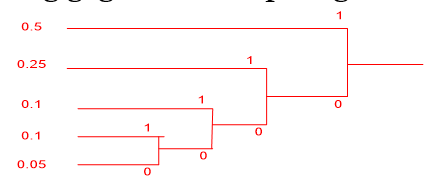
\includegraphics[width=.5\linewidth]{./01-quellencodierung/optimierung_codierung}
    \vspace{-8pt}
\end{center}

\begin{center}
    \centering
    \begin{tabular}{l | l}
        \bfseries{Zeichen} & \bfseries{Huffman}\\ \hline
        a & 1\\ 
        b & 01\\
        c & 001\\
        d & 0001\\
        e & 0000\\
    \end{tabular}
\end{center}

Daraus folgt für die Redundanz nach Huffman = 0.02. 
Das sind 11.8\% und entspricht einer Redundanzreduktion um 88.2\%.

\subsubsection{C}
Der Informationsgehalt einer Bildvorlage soll über einen Binärkanal mit der Kanalkapaziät von 40 kBit/sec übertragen werden. Dabei wird das Bild durch Abtastung in 105 Bildpunkte zerlegt. Ein Bild-punkt kann in 8 Helligkeitswerte H zerlegt werden.

\paragraph{Welche Übertragungszeit ergibt sich, wenn alle Helligkeitswerte gleich codiert werden?}\mbox{}\\
$L_D 8=3$ Bit pro Bildpunkt\\
$\rightarrow TÜ = 3*10^5:40kBit/sec=7.5sec$\\

Nähere Untersuchungen der Helligkeitswerte ergeben für die Helligkeitswerte H1 bis H8 folgende Ver-teilung ihrer Auftrittswahrscheinlichkeit:
\begin{center}
    \centering
    \begin{tabular}{l | l}
        \bfseries{H} & \bfseries{P}\\ \hline
        H1 & 0.4\\ 
        H2 & 0.35\\
        H7 & 0.1\\
        H4 & 0.0625\\
        H3 & 0.035\\
        H5 & 0.03225\\
        H6 & 0.01425\\
        H8 & 0.006
    \end{tabular}
\end{center}

\paragraph{Um wie viel Prozent können sie die Übertragungsgeschwindigkeit eines Bildes verkürzen, wenn sie die erfassten Bildpunkte vor dem Versenden nach Huffmann codieren?}\mbox{}\\
\begin{center}
    \centering
    \begin{tabular}{p{1cm} | p{1cm} | p{1cm} | p{1cm} | p{1cm}}
        \bfseries{H} & \bfseries{P} & \bfseries{Möglicher Code} & \bfseries{Anzahl Bits} & \bfseries{Länge}\\ \hline
        H1 & 0.4 & 0 & 1 & 0.4\\ 
        H2 & 0.35 & 10 & 2 & 0.7\\
        H7 & 0.1 & 110 & 3 & 0.3\\
        H4 & 0.0625 & 1110 & 4 & 0.25\\
        H3 & 0.035 & 11110 & 5 & 0.175\\
        H5 & 0.03225 & 111110 & 6 & 0.1935\\
        H6 & 0.01425 & 1111110 & 7 & 0.09975\\
        H8 & 0.006 & 1111111 & 7 & 0.042\\
        Total & & & & 2.16025
    \end{tabular}
\end{center}

$TÜ=2.16*10^5:40kBit/sec = 5.4sec$\\
$7.5=100\%$\\
$5.4 = 5.4/7.5*100\% = 72\%$\\
Daraus folgt eine Verbesserung um 28\%.

\paragraph{Für den Kanal konnte die folgende Kanalmatrix P(Y|X) ermittelt werden.}\mbox{}\\
$P(X|Y) = \begin{matrix}
    0.9 & 0.1\\
    0.1 & 0.9\\
\end{matrix}$

Wie lange dauert es dann mindestens, bis alle Daten fehlerfrei übertragen sind? Gehen Sie davon aus das „0“ und  „1“ gleich wahrscheinlich sind. \\
$TÜ = 2.16*10^5:(1000*40Bit)=5.4sec$

\subsection{Huffman}
\subsubsection{A}
Gegeben sind die folgenden Zeichen a, b, c, d mit den Auftrittswahrscheinlichkeiten 
P{a} = 0.5, P{b}= 0.25, P{c} = 0.125, P{d}= 0.125\\

Zeigen Sie, dass eine nach Huffmann codierte Quellencodierung einen Redundanzfreien 
Code ergibt.
\begin{center}
    \vspace{-8pt}
    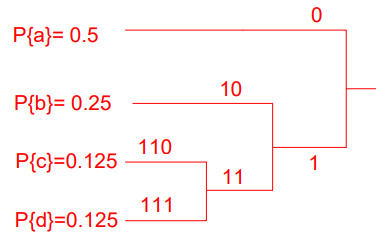
\includegraphics[width=.5\linewidth]{./01-quellencodierung/hs2009}
    \vspace{-8pt}
\end{center}

$H(X) = 0.5*log_2(\frac{1}{0.5})+0.25*log_2(\frac{1}{0.25})+0.125*log_2(\frac{1}{0.125})=1.75$\\
$L=0.5*1+0.25*2+0.125*3+0.125*3=1.75$\\
$R_c=L-H(x)=0$

\subsubsection{B}
Codieren Sie die nachfolgenden Zeichen mit der Huffmancodierung\\
\textit{ABRAKADABRA}\\

\paragraph{Auftrittswahrscheinlichkeit pro Zeichen}\mbox{}\\
$\frac{Häufigkeitsverteilung Zeichen}{Anzahl Symbole}$

\begin{center}
    \centering
    \begin{tabular}{p{1.9cm} | p{0.5cm} | p{0.5cm} | p{0.5cm} | p{0.5cm} | p{0.5cm} }
        \bfseries{Symbol} & \bfseries{A} & \bfseries{B} & \bfseries{R} & \bfseries{K} & \bfseries{D}\\ \hline
        Häufigkeitsvert. & 5 & 2 & 2 & 1 & 1\\ 
        p(Symbol) & 0.45 & 0.18 & 0.18 & 0.09 & 0.09
    \end{tabular}
\end{center}

\paragraph{Informationsgehalt pro Zeichen}\mbox{}\\
$I(x)=log_2(\frac{1}{p(x)}) \rightarrow [I(x)]=bit$

\begin{center}
    \centering
    \begin{tabular}{p{1.9cm} | p{0.5cm} | p{0.5cm} | p{0.5cm} | p{0.5cm} | p{0.5cm} }
        \bfseries{Symbol} & \bfseries{A} & \bfseries{B} & \bfseries{R} & \bfseries{K} & \bfseries{D}\\ \hline
        Häufigkeitsvert. & 5 & 2 & 2 & 1 & 1\\ 
        I(x) & 1.37 & 2.45 & 2.45 & 3.45 & 3.45
    \end{tabular}
\end{center}

\paragraph{Huffmancodierung}\mbox{}\\
% TODO:

\subsection{Diskrete Quelle mit Gedächtnis}
\subsubsection{A}
Ein Code hat die durch das angegebene Markoffdiagramm gegeben inneren Abhängigkeiten.\\

Ergänzen Sie die fehlenden Wahrscheinlichkeitswerte im Diagramm.
\begin{center}
    \vspace{-8pt}
    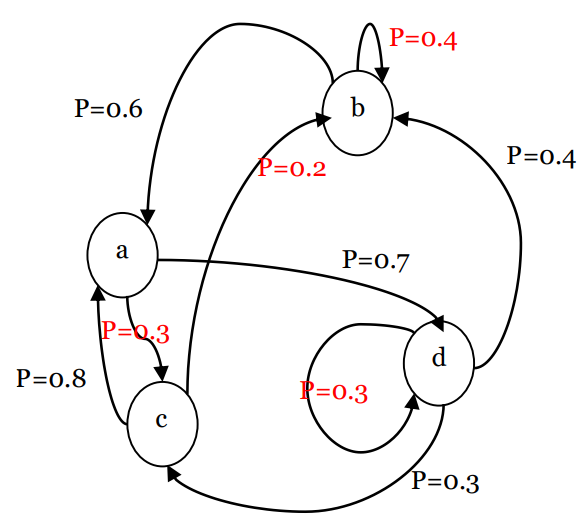
\includegraphics[width=.5\linewidth]{./01-quellencodierung/hs2009_1}
    \vspace{-8pt}
\end{center}

Bestimmen Sie die Entropie des Codes H(X) sowie die Verbundentropie H(X|Y). Um wieviel Prozent kann die Redundanz gesenkt werden, wenn die inneren Abhängigkeiten berücksichtigt werden?\\
% TODO: Schritte über TI-Nspire beschreiben & wo ablesen

\subsubsection{B}
Sie untersuchen eine diskrete Quelle mit Gedächtnis. Die Quelle hat den folgenden Zeichensatz: A, B, C\\
Die bedingte Wahrscheinlichkeit ist gegeben:\\
$\begin{matrix}
    P(A|A) & P(B|A) & P(C|A)\\
    P(A|B) & P(B|B) & P(C|B)\\
    P(A|C) & P(B|C) & P(C|C)
\end{matrix} = \begin{matrix}
    0 & 1/5 & 8/10\\
    1/10 & 1/2 & 2/5\\
    9/20 & 1/2 & 1/20
\end{matrix}$

Zeichnen Sie das Markoff-Diagramm.
\begin{center}
    \vspace{-8pt}
    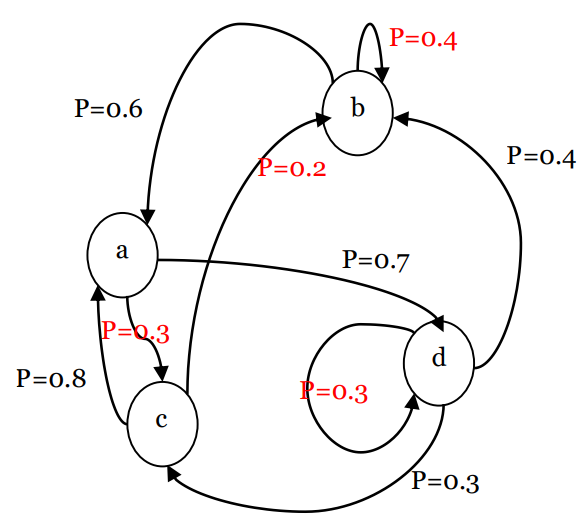
\includegraphics[width=.5\linewidth]{./01-quellencodierung/hs2009_1}
    \vspace{-8pt}
\end{center}

\columnbreak

\subsection{Lempel-Ziv}
\subsubsection{A}
Codieren Sie die nachfolgende Bitfolge mit dem Lempel-Ziv 77 Verfahren:\\
$01101110101010001101110$
\begin{center}
    \vspace{-8pt}
    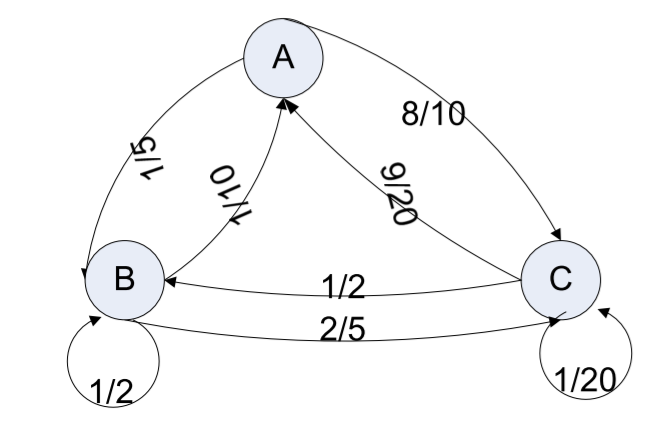
\includegraphics[width=.8\linewidth]{./01-quellencodierung/hs2009_2}
    \vspace{-8pt}
\end{center}

Bestimmen Sie die Auftrittswahrscheinlichkeiten der Zeichen\\
$P(A)=iP(B)+1/10+P(C)*9/20$\\
$P(B)=P(A)*1/5+P(B)*1/2+P(C)*1/2$\\
$P(C)=P(A)*8/10+P(B)*2/5+P(C)*1/20$\\
$1=P(A)+P(B)+P(C)$\\

$P(A)=\frac{55}{269}=0.20$\\
$P(B)=\frac{118}{269}=0.43$\\
$P(C)=\frac{96}{269}=0.34$







        %! Licence = CC BY-NC-SA 4.0

%! Author = gianfluetsch
%! Date = 22. Jan 2022
%! Project = icth_summary

\section{Verschlüsselung}
\subsubsection{A}
Mit RSA-verschlüsselte Nachricht c=8 abgefangen und kennen öffentlichen Schlüssel des Empfängers (e=13, n=323).
Aus sicherer Quelle wissen Sie, dass eine der beiden Primzahlen 17 ist. Entschlüsseln Sie die Nachricht!\\
Gegeben: $c=8, e=13, n=323, p=17$\\
$solve(323=17*x,x) \rightarrow q=19$\\
$\phi(n) = (p-1)*(q-1) = 16*18=288$\\
$d=\frac{2*\phi(n)+1}{e}=\frac{2*288+1}{13}$\\
$d=rsa\_ereuk(17,288) \rightarrow d=17$\\
$rsa\_dec(8,13,323) \rightarrow m=179$\\
$\rightarrow$ d negativ $\rightarrow$ d=Wert in obiger Spalte nehmen

\subsubsection{B}
Mit RSA-verschlüsselte Nachricht c=4 abgefangen und kennen öffentlichen Schlüssel des Empfängers (e=13, n=143).
Beide Primzahlen (p \& q) sind grösser als 10. Entschlüsseln Sie die Nachricht!\\
Gegeben: $c=8, e=13, n=143$\\
$p=11, q=13 \rightarrow 11*13 = 143$\\
$\phi(n) = (p-1)*(q-1) = 10*12=120$\\
$d=\frac{2*\phi(n)+1}{e}=\frac{2*288+1}{13}$\\
$d=rsa\_ereuk(13,120) \rightarrow d=37$\\
$rsa\_dec(4,13,143) \rightarrow m=108$

\subsubsection{C}
Es wird ein asymmetrisches Verfahren (RSA) verwendet. Wie viele verschiedene Schlüsselpaare müssen erzeugt werden, wenn in einer Gruppe von 25 Teilnehmern. jeder mit jedem vertraulich kommunizieren möchte?\\
\textit{25 Schlüsselpaare}\\

Wie viele Schlüssel muss jeder Teilnehmer speichern, wenn sie davon ausgehen, dass es eine vertrauenswürdige „Schlüsselbank“ gibt, bei der die öffentlichen Schlüssel abgefragt werden können?\\
\textit{Bei einer öffentlichen Schlüsselbank. Nur seinen Private Key (und ggf. noch seinen öffentlichen).}\\

Teilnehmer a möchte an Teilnehmer b eine verschlüsselte und signierte Nachricht versenden. Welche Schlüssel verwendet
\begin{itemize}
    \item User a: \textit{public Key von b und private Key von a}
    \item User b: \textit{public Key von a und private Key von b}\\
\end{itemize}

Kommt es bei der Anwendung durch die Teilnehmer a und b dabei auf die Reihenfolge der Schlüssel an?\\
\textit{Nein}\\

\paragraph{Gegeben seien die beiden Primzahlen 11 und 5}\mbox{}\\
Bestimmen sie die Zahl \textit{n} und die Zahl $\phi(n)$\\
$n=11*5=55$\\
$\phi(n) = 10*4=40$

\paragraph{Zur Verschlüsselung wird der öffentliche Schlüssel e  = 17 verwendet}\mbox{}\\
Ermitteln sie den privaten Schlüssel d zum Entschlüsseln einer Nachricht.\\
Es muss gehlten: $e*dmod\phi(n)=1$\\

\begin{center}
    \vspace{-8pt}
    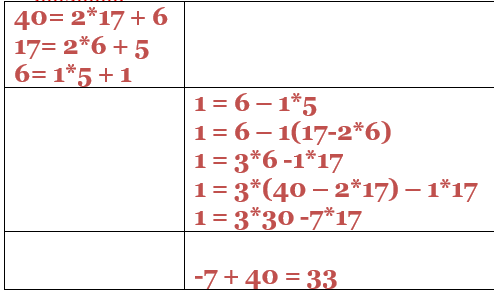
\includegraphics[width=.7\linewidth]{./01-quellencodierung/fs2017_4}
    \vspace{-8pt}
\end{center}

$rsa\_euklid(17,40)$\\

Daraus folgt, 33 ist die Inverse zu 17 bzgl. der mod40 Rechnung. D.h. der Schlüssel zum Entschlüsseln ist 33.

\subsubsection{D}
91 Teilnehmer wollen paarweise vertraulich Informationen austauschen.\\

In einem ersten Ansatz wird ein symmetrisches Verfahren gewählt. 
Wie viele verschiedene Schlüssel müssen erzeugt werden, wenn jeder mit jedem vertraulich kommunizieren möchte?\\
$91/2*90=4095$ oder $nCr(91,2)=4096$\\

Wie viele Schlüssel muss jeder Teilnehmer speichern?\\
\textit{N=90}\\

\subsubsection{E}
Handel es sich bei der Cesar-Verschlüsselung um ein symmetrisches oder asym-metrisches Verfahren?\\
\textit{Um ein symmetrisches Verfahren}\\

Wird bei diesem Verfahren jedes Quellzeichen einzeln Verschlüsselt oder werden immer mehrere Quellzeichen zur Verschlüsselung zusammengefasst?\\
\textit{Es wird jedes Quellzeichen einzeln codiert}\\

Beschreiben Sie, wie sie in diesem Fall eine einfache Kryptoanalyse machen können und was sie dazu brauchen?\\
\textit{Bei einer Cesar-Verschlüsselung werden die Häufigkeiten der Quellzeichen nicht verwürfelt. Ist die Zielsprache bekannt ist auch das häufigste Zeichen der Spra-che bekannt. Ist der Erhaltene Code gross genug kann mit einer einfachen Häu-figkeitsanalyse der Schlüssel ermittelt werden.}\\

\columnbreak

Gegeben seien die beiden Primzahlen 15 und 11. Als öffentlichen Schlüssel wählen Sie die Primzahl 17.\\
Berechnen sie den inversen, privaten Schlüssel und machen sie alle Zwischenschritte deutlich.\\
$n = 143 \rightarrow \phi(n)=12*10=120$\\
Es muss gelten: $e*d mod \phi(n) = 1$\\
$120=17*7+1$\\
$7=1*7+0$\\

$1=120-17*7$\\
$1=-17*7mod120 + 120 * 7$\\
$1=103*7mod120$\\
$7^{-1}mod120=113$\\

$rsa\_euklid(17,120) \rightarrow d=113$\\

Daraus folgt, 113 ist der Inverse Schlüssel.\\

Verschlüsseln Sie die Zahl 3 mit dem öffentlichen Schlüssel 17, mache sie die Rechenschritte deutlich.\\
$=3^{17}mod143$\\
$=3^{10}*3^7mod143$\\
$=9$\\

$rsa\_enc(3,17,143) \rightarrow 9$\\

Welchen Schlüssel verwenden sie, um eine Nachricht zu:\\
\begin{itemize}
    \item Unterschreiben: \textit{eigenen private Key}
    \item Verschlüsseln: \textit{public Key vom Empfänger}
\end{itemize}
        %! Licence = CC BY-NC-SA 4.0

%! Author = gianfluetsch
%! Date = 22. Jan 2022
%! Project = icth_summary

\section{Kanalcodierung}

\subsection{Blockcode}
\subsubsection{Nachprüfung HS2020}
$x_5=x_1+x_2+x_3$\\
$x_6=x_1+x_2+x_4$\\
$x_7=x_2+x_3+x_4$

\paragraph{Prüfmatrix des Blockcodes}\mbox{}\\
$\begin{matrix}
    x_1 & x_2 & x_3 & x_4 & | & x_5 & x_6 & x_7\\
    1 & 1 & 1 & 0 & | & 1 & 0 & 0\\
    1 & 1 & 0 & 1 & | & 0 & 1 & 0\\
    0 & 1 & 1 & 1 & | & 0 & 0 & 1
\end{matrix}$

\paragraph{Anzahl Kontrollstellen}\mbox{}\\
Anzahl Kontrollstellen = Anzahl 1 in Prüfmatrix (Einheitsmatrix) $\rightarrow$ 3

\paragraph{Anzahl gültige Codeworte mit Blockcode}\mbox{}\\
gültige Codeworte = Anzahl Spalten ohne Prüfmatrix\\
$m=4 \rightarrow 2^m=2^4=16$

\paragraph{Fehlersyndom, falls x1 und x2 gestört}\mbox{}\\
$110$\\
$111$\\
$--$\\
$001$

\paragraph{Fehler erkennen}\mbox{}\\
Ja, der Fehler (Syndrom) liegt in der Spalte $x_7$ der Prüfmatrix.
Geht man nun davon aus, dass nur ein Fehler passiert ist, so wird man hier eine Falschkorrektur vornehmen
(durch flippen des siebten Bits)

\paragraph{Fehler korrigieren?}\mbox{}\\
Nein, Fehler kann nicht korrigiert werden, da er in der regulären Prüfmatrix nicht gefunden wurde.

\subsubsection{Prüfung Fs2017}
Gegeben ist die folgende Generatormatrix eines systematischen Blockcodes mit den Prüfvektoren $p_1$ bis $p_7$:
$\begin{matrix}
    p_1 & p_2 & p_3 & p_4 & p_5 & p_6 & p_7\\
    1 & 0 & 1 & 1 & 0 & 0 & 0\\
    1 & 1 & 1 & 0 & 1 & 0 & 0\\
    1 & 1 & 0 & 0 & 0 & 1 & 0\\
    0 & 1 & 1 & 0 & 0 & 0 & 1
\end{matrix}$

\paragraph{Wie viele Nachrichtenstellen m hat der Code?}\mbox{}\\
Code hat 3 Nachrichtenstellen

\paragraph{Wie viele Kontrollstellen k hat der Code?}\mbox{}\\
Der Code hat 4 Kontrollstellen

\paragraph{Wie lautet das Fehlersyndrom, wenn nur das dritte Bit einer Nachricht falsch übertragen wird?}\mbox{}\\
101

\paragraph{Ermitteln Sie die Hamming-Distanz des Codes}\mbox{}\\
$H=4$\\
Es müssen mindestens 4 Prüfvektoren addiert werden, um den Orginalen-Vektor zu erhalten.

\paragraph{Ist der Code dicht gepackt?}\mbox{}\\
Der Code ist nicht dichtgepackt, da $H=4$ ist. Damit liegt mindestens 1 Codewort (CW) ausserhalb \textit{einer Korrigierkugel}.

\subsubsection{Prüfung FS2015}
Gegeben ist die folgende Prüfmatrix eines  Hamming Blockcode
\begin{center}
    \vspace{-8pt}
    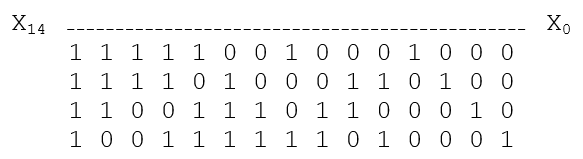
\includegraphics[width=.7\linewidth]{./02-kanalcodierung/fs2015_1}
    \vspace{-8pt}
\end{center}

Wie gross ist die
\begin{itemize}
    \item Anzahl der Kontrollstellen: $k=4$
    \item Anzahl Nachrichtenstellen: $m=2^4-1-k=11$
    \item Codewortlänge CW: $2^4-1=15$
    \item Anzahl korrigierbare Fehler: $1$
    \item Anzahl gültige Codeworte: $2^11=2048$\\
\end{itemize}

Bestimmen sie für den Fall, dass die Codestellen x13 und x11 fehlerhaft sind das Fehlersyndrom?\\
Syndrom $(0011)^T$\\

Was würde bei einer Vorwärtskorrektur passieren?\\
\textit{x6 würde fälschlicherweise Korrigiert.}

\subsubsection{Prüfung HS2009}
Gegeben sind die folgenden Fehlersyndrome für einen einzigen Bitfehler an der jeweiligen Stelle xi eines systematischen Blockkodes:\\
$Z(x1)=[111], Z(x2)=[110], Z(x3)=[101], Z(x4)=[011], Z(x5)=[100], Z(x6)=[010], Z(x6)=[001]$\\

Geben Sie die Generatormatrix des Blockcodes an.\\
$\begin{matrix}
    x1 & x2 & x3 & x4 & x5 & x6 & x7\\
    1 & 1 & 1 & 0 & 1 & 0 & 0\\
    1 & 1 & 0 & 1 & 0 & 1 & 0\\
    1 & 0 & 1 & 1 & 0 & 0 & 1
\end{matrix}$

Wie gross ist die Hammingdistanz des Codes?\\
$h=3$\\
% TODO: Hamming-Distanz = Anzahl Kontrollstellen?

Ermittelten sie für die unten aufgeführten Nachrichtenwörter die vollständigen Codewörter\\
$NW1 = x6 = 0001$ $\textcolor{red}{0}$ $\textcolor{red}{1}$ $\textcolor{red}{1}$\\
$NW2 = x7 = 1010$ $\textcolor{red}{0}$ $\textcolor{red}{1}$ $\textcolor{red}{0}$

\subsubsection{Prüfung FS2009}
Gegeben ist die folgende Generatormatrix.
\begin{center}
    \vspace{-8pt}
    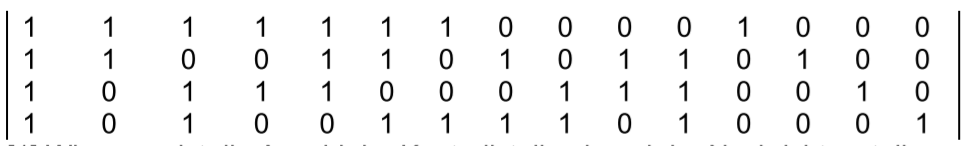
\includegraphics[width=.8\linewidth]{./02-kanalcodierung/fs2009_2}
    \vspace{-8pt}
\end{center}

Wie gross ist die Anzahl der Kontrollstellen k und der Nachrichtenstellen m?\\
$k=4, m=11$\\

Sie empfangen die folgenden Codewörter.
\begin{center}
    \vspace{-8pt}
    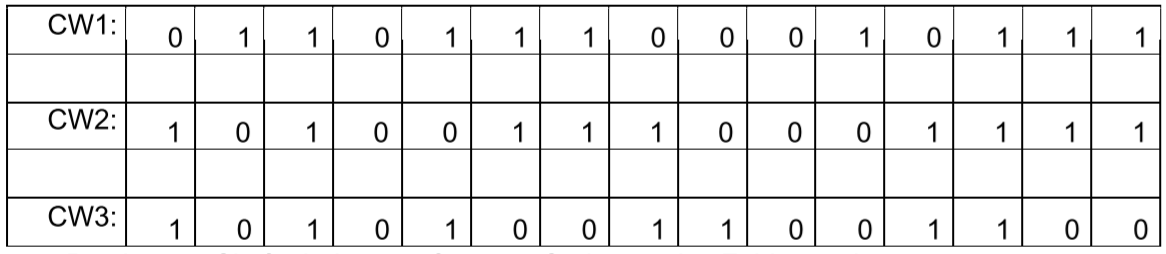
\includegraphics[width=.8\linewidth]{./02-kanalcodierung/fs2009_3}
    \vspace{-8pt}
\end{center}

\begin{itemize}
    \item Bestimmen Sie für jedes empfangene Codewort das Fehlersyndrom.
    \item Bestimmen sie ferner, welche Codewörter wahrscheinlich korrekt und welche fehlerhaft übertragen wurden.
    \item Im Fehlerfall geben Sie bitte an, welche Stelle voraussichtlich gestört wurde.
\end{itemize}
\textit{CW1: 1 1 0 1, Fehlerposition: x6}\\
\textit{CW2: 1 0 1 0, Fehlerposition: x4}\\
\textit{CW3: kein Fehler!}\\

Konstruieren Sie einen (reduzierten) Hamming-Code (Generatormatrix) für den Fall, dass Sie 8-stellige Nachrichten gegen Übertragungsfehler absichern müssen. Warum spricht man von einem reduzierten Code?\\
\begin{center}
    \vspace{-8pt}
    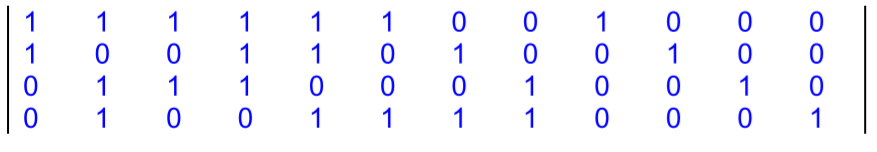
\includegraphics[width=.8\linewidth]{./02-kanalcodierung/fs2009_4}
    \vspace{-8pt}
\end{center}
\textit{Reduzierter Code: Weil die Anzahl der Nachrichtenstellen nicht vollständig ausgenutzt werden.}

\subsection{Zyklischer Code}
\subsubsection{Nachprüfung HS2020}
Gegeben ist folgendes Generatorpolynom:
$p(x)=x^5+x^3+x^2+1$

\paragraph{Wie viele Kontrollstellen hat Code}\mbox{}\\
Grad 5 $\rightarrow$ 5 Kontrollstellen

\paragraph{Schieberegister}\mbox{}\\
\begin{center}
    \vspace{-8pt}
    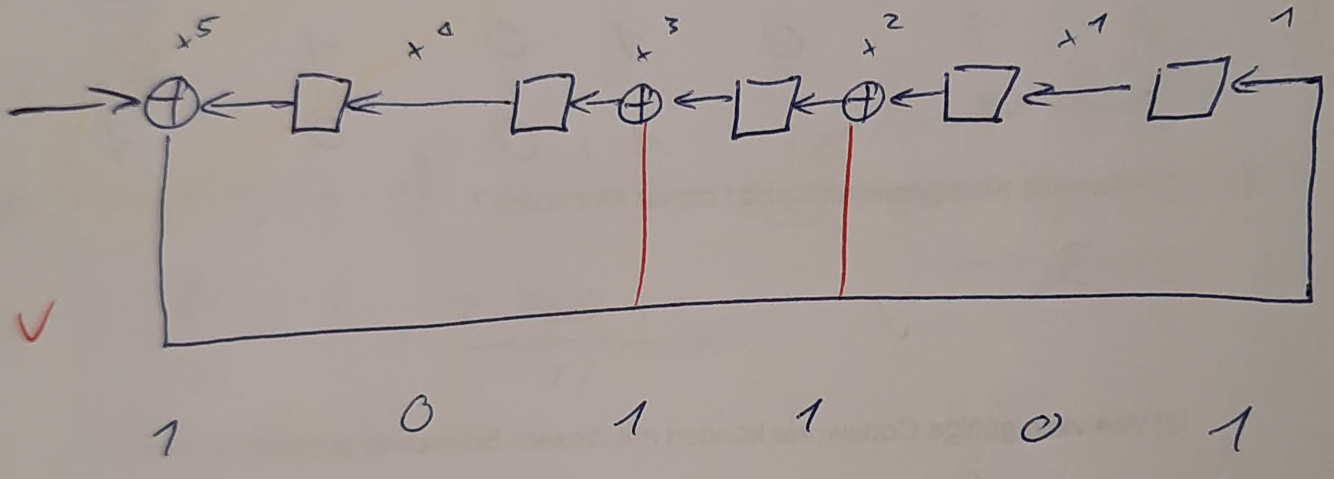
\includegraphics[width=.8\linewidth]{./02-kanalcodierung/schieberegister}
    \vspace{-8pt}
\end{center}

\paragraph{Prüfen, ob Codewort gültig}\mbox{}\\
Prüfmatrix aus Schieberegister ablesen (101101).
\begin{center}
    \vspace{-8pt}
    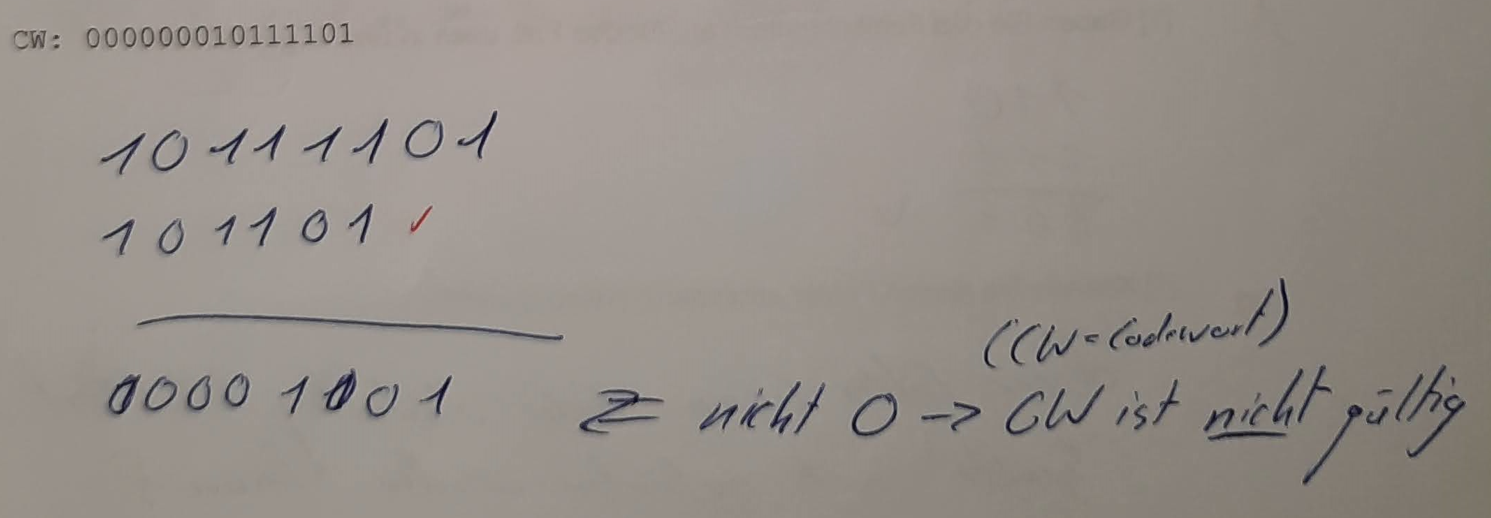
\includegraphics[width=.8\linewidth]{./02-kanalcodierung/codewort}
    \vspace{-8pt}
\end{center}

\paragraph{Fehlersyndrom für Stelle $x^5$ mit Polynomdivison ermitteln}\mbox{}\\
$x^5:x^3+x^2+1 \rightarrow Rest: x+1$

\subsubsection{Prüfung FS2017}
Gegeben ist das folgende Generatorpolynom:\\
$g(x)=x^4+x^3+x^2+1$

\paragraph{Ist das Generatorpolynom irreduzibel?}\mbox{}\\
\begin{center}
    \vspace{-8pt}
    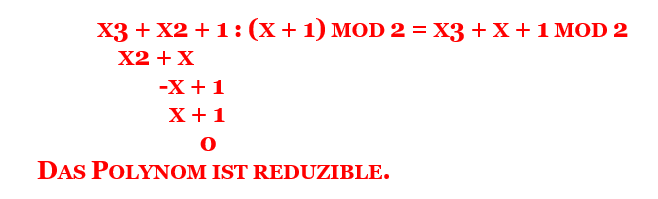
\includegraphics[width=.8\linewidth]{./02-kanalcodierung/fs2017}
    \vspace{-8pt}
\end{center}

\paragraph{Ermitteln Sie die Kontrollstellen für die Nachricht m=100}\mbox{}\\
\begin{center}
    \vspace{-8pt}
    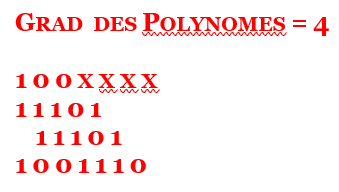
\includegraphics[width=.5\linewidth]{./02-kanalcodierung/fs2017_1}
    \vspace{-8pt}
\end{center}

\paragraph{Ermitteln Sie die Zyklusfolge des Polynoms}\mbox{}\\
$A4+A3+A2=1$\\
$0,(1=A0),A,A2,A3$\\

$A4=A3+A2+1$\\

$A5 = A4 + A3 + A = A3 + A2 + 1 +  A3 + A =  A2 + A + 1$\\
$A6= A3 + A2 + A$\\
$A7= A4 + A3 + A2 = A3 + A2 + 1 + A3 + A2 = 1$\\
Somit ergibt sich der Zyklus zu: 0001, 0010, 0100, 1000, 1101, 1110, 0001

\subsubsection{Prüfung FS2015}
Gegeben ist das folgende Generatorpolynom p:\\
$p(x)=1+x^2+x^6+x^{10}+x^{14}$\\

Prüfen Sie durch Rechnung, ob das Polynom irreduzibel ist.
\begin{center}
    \vspace{-8pt}
    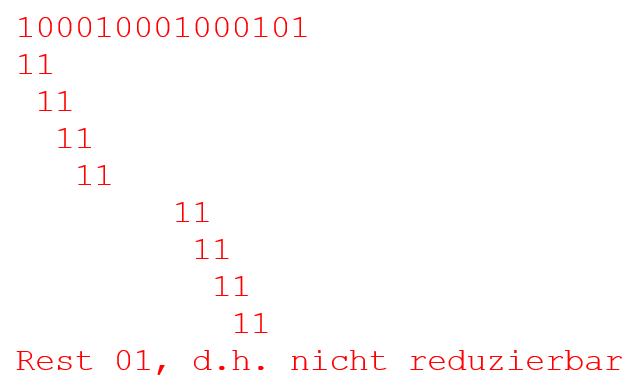
\includegraphics[width=.5\linewidth]{./02-kanalcodierung/fs2015_2}
    \vspace{-8pt}
\end{center}

Wie gross sind in diesem Fall
\begin{itemize}
    \item Kontrollstellenzahl (k): $k=14$
    \item Nachrichtenzahl (m): $m=2^{14}-1-14=16369$
    \item Codewortlänge (n): $n=2^{14}-1=16383$
\end{itemize}

\subsubsection{Prüfung HS2009}
Gegeben ist das folgende Generatorpolynome p\\
$p(x)=1+x^2+x^4+x^5$\\

Wie gross ist die Anzahl der Nachrichtenstellen m, die Kontrollstellen k sowie die Hammingdistanz h? (Achtung: Ist das Polynom prim?)\\
Das Polynom ist nicht prim:\\
$(x^5+x^4+x^2+1):(x+1)=(x^4+x+1)(x+1)$\\
d.h. $h=4,k=5,n=2^4-1=15 \rightarrow m=10$\\

Prüfen sie, ob das Generatorpolynom $p_1(x)=1+x+x^4+x^5$ das folgende Codewort gültig ist.\\
\begin{center}
    \vspace{-8pt}
    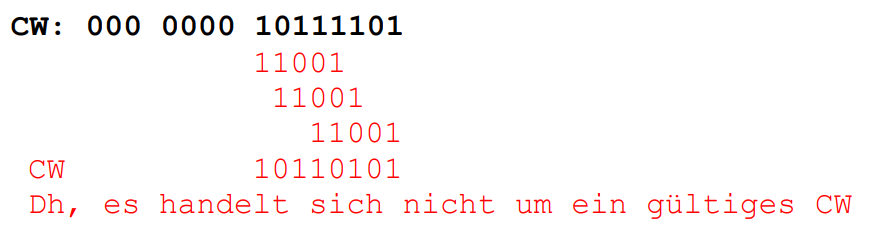
\includegraphics[width=.5\linewidth]{./02-kanalcodierung/hs2009_2}
    \vspace{-8pt}
\end{center}

\subsubsection{Prüfung FS2009}
Gegeben sind die folgenden Generatorpolynome p1 und p2:\\
$p_1(x)=1+x+x4$\\
$p_2(x)=1+x2+x4+x5$\\

Zeigen Sie, dass ein Generatorpolynom einen Hamming-Code und das andere einen Abramson-Code darstellt.\\
\textit{Hamming-Code: p1 nicht weiter teilbar}\\
\textit{Abramson-Code: p2, p1*(1+x)}\\

Wie gross ist jeweils die Anzahl der Nachrichtenstellen m, die Kontrollstellen k sowie die Hammingdistanz h?\\
$p_1: k=4, m=11, h=3$\\
$p_2: k=5, m=10, h=4$\\

Geben Sie für das Generatorpolynom p1(x)=1+x+x4 das rückgekoppelte Schieberegister zur Ermittlung der Kontrollstellen an.
\begin{center}
    \vspace{-8pt}
    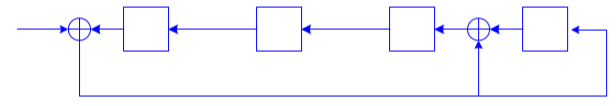
\includegraphics[width=.7\linewidth]{./02-kanalcodierung/fs2009_5}
    \vspace{-8pt}
\end{center}

Geben Sie mit Hilfe des Schieberegisters an, ob das folgende Codewort gültig ist (Weg muss ersichtlich sein). CW: 000 0000 1011 1101
\begin{center}
    \vspace{-8pt}
    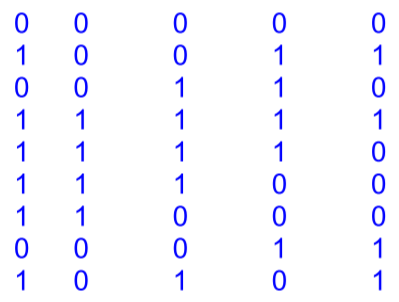
\includegraphics[width=.3\linewidth]{./02-kanalcodierung/fs2009_6}
    \vspace{-8pt}
\end{center}

\subsection{Faltungscode}
\subsubsection{Nachprüfung HS2020}\mbox{}\\
\begin{center}
    \vspace{-8pt}
    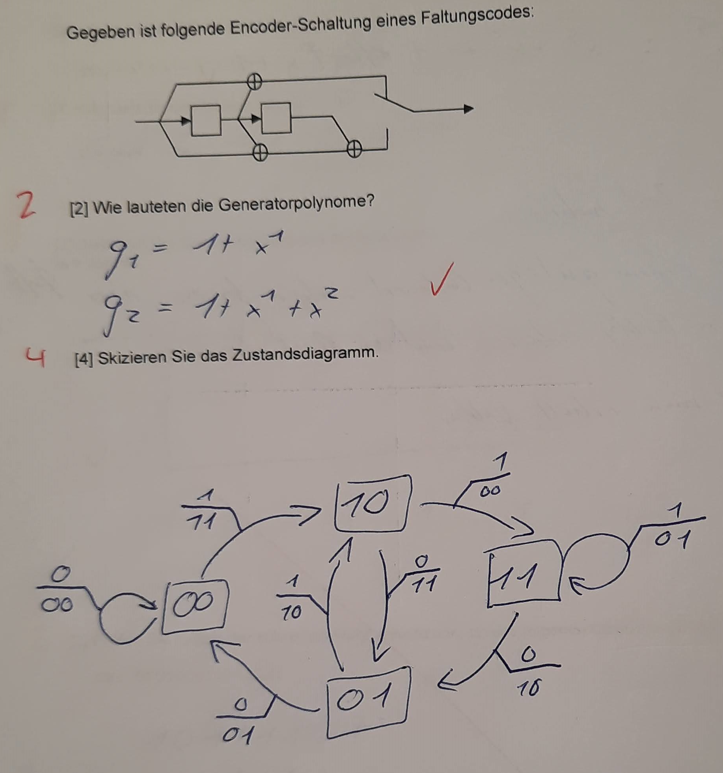
\includegraphics[width=.8\linewidth]{./02-kanalcodierung/faltungscode}
    \vspace{-8pt}
\end{center}

\subsubsection{Prüfung FS2017}
Gegeben ist der folgende Faltungscodierer
\begin{center}
    \vspace{-8pt}
    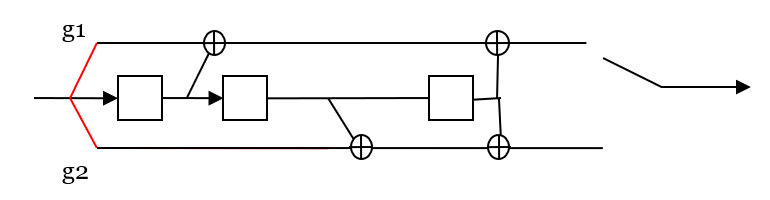
\includegraphics[width=.8\linewidth]{./02-kanalcodierung/fs2017_2}
    \vspace{-8pt}
\end{center}

\paragraph{Wie viele Bits werden zur Berechnung der Ausgangsbit herangezogen?}\mbox{}\\
4, drei aus dem Speicher und das aktuelle


\paragraph{Bestimmen Sie die Impulsantwort der Decoderschaltung}\mbox{}\\
\begin{center}
    \vspace{-8pt}
    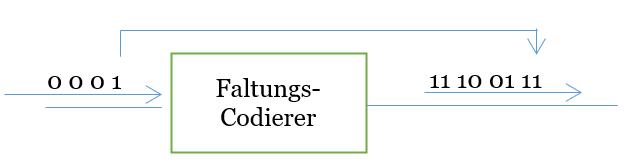
\includegraphics[width=.8\linewidth]{./02-kanalcodierung/fs2017_3}
    \vspace{-8pt}
\end{center}

\paragraph{Geben Sie die Codes in Polynomdarstellung an}\mbox{}\\
$g_1=x^3+x+1$\\
$g_2=x^3+x^2+1$

\paragraph{Wie viele Zustände hat der Coder?}\mbox{}\\
8

\paragraph{Bestimmen Sie seine Coderate}\mbox{}\\
$\frac{Anzahl Ausgangsbits}{Anzahl Eingangsbits} = \frac{8}{4}=2$\\

\subsubsection{Prüfung HS2016}
Gegeben seien die folgenden Impulsantworten eines (3,1,2)-Faltungscodierers:\\
${g_1}={1,1,0}, {g_2}={1,0,1} \& {g_3}={1,1,1}$\\

\paragraph{Zeichnen Sie die Encoder Schaltung}\mbox{}\\
\begin{center}
    \vspace{-8pt}
    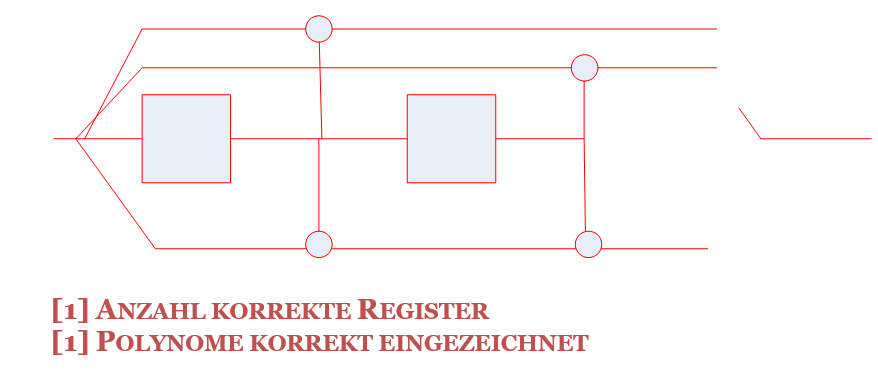
\includegraphics[width=.8\linewidth]{./02-kanalcodierung/hs2016}
    \vspace{-8pt}
\end{center}

\paragraph{Wie viele Tail-Bits müssen einer Nachrichtenfolge angefügt werden?}\mbox{}\\
2 TAIL-BITS

\paragraph{Geben Sie das Encoder-Zustandsdiagramm an}\mbox{}\\
\begin{center}
    \vspace{-8pt}
    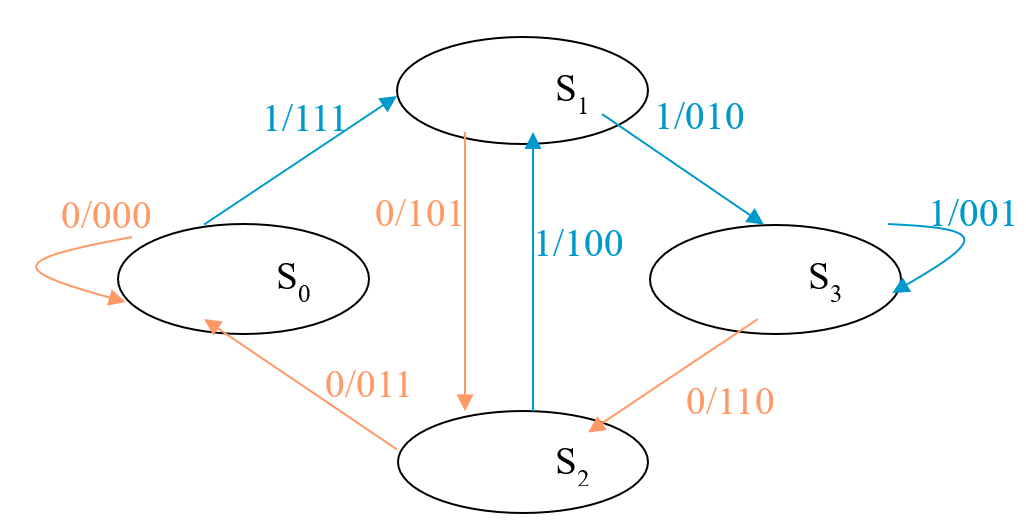
\includegraphics[width=.8\linewidth]{./02-kanalcodierung/hs2016_1}
    \vspace{-8pt}
\end{center}

\paragraph{Liegt ein katastrophaler Code vor (Begründung)?}\mbox{}\\
Nein, da es keine Zyklen ohne Gewichtszunahme gibt.

\paragraph{Bestimmen sie die (Block)-Coderate}\mbox{}\\
$B=Eingabebits$\\
$R=\frac{B}{N} = \frac{B}{3*(B+2)}$

\subsubsection{Prüfung HS2009}
Gegeben seien die folgenden Impulsantworten eines Faltungscodierers mit einem Eingang:\\
${g1}={1,1,0}$ und ${g2}={1,1,1}$\\

Zeichen Sie die Encoder Schaltung.
\begin{center}
    \vspace{-8pt}
    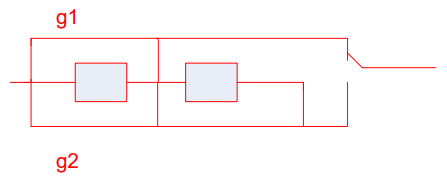
\includegraphics[width=.8\linewidth]{./02-kanalcodierung/hs2009_3}
    \vspace{-8pt}
\end{center}

Wie viele Tail-Bits müssen einer Nachrichtenfolge angefügt werden?\\
\textit{2 Tailbits}\\

Geben Sie das Encoder-Zustandsdiagramm an.\\
\begin{center}
    \vspace{-8pt}
    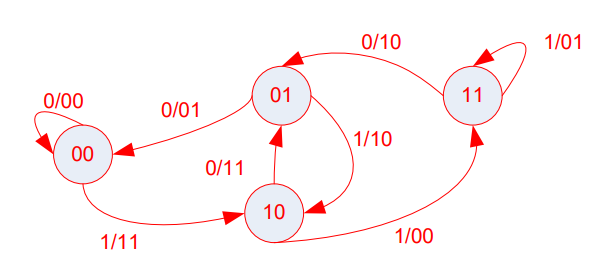
\includegraphics[width=.8\linewidth]{./02-kanalcodierung/hs2009_4}
    \vspace{-8pt}
\end{center}

Handelt es sich um einen „Guten Code“ (Mit Begründung)?\\
\textit{Ja, da der Unterschied der Ausgabe bei einem Zustandsübergang immer maximal ist.}\\

Ermitteln Sie für die Nachrichtenfolge ${u[n]}={1,0,1,1,0,1,1}$ die Ausgangscodefolge {v[n]}.\\
\begin{center}
    \vspace{-8pt}
    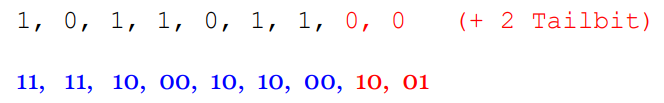
\includegraphics[width=.8\linewidth]{./02-kanalcodierung/hs2009_5}
    \vspace{-8pt}
\end{center}

\subsubsection{Prüfung FS2009}
Gegeben seien die folgenden Impulsantworten eines (2,1,2)-Faltungscodierers: {g1}={1, 1, 0} und {g2}={1, 0, 1}\\

Zeichnen Sie die Encoder-Schaltung.
\begin{center}
    \vspace{-8pt}
    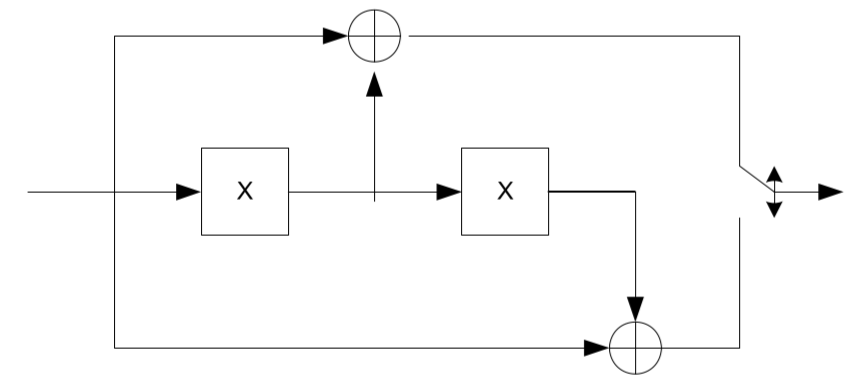
\includegraphics[width=.8\linewidth]{./02-kanalcodierung/fs2009_7}
    \vspace{-8pt}
\end{center}

Wie viele Tail-Bits müssen einer Nachrichtenfolge angefügt werden?\\
\textit{2 Tail-Bits}\\

Geben Sie das Encoder-Zustandsdiagramm an.
\begin{center}
    \vspace{-8pt}
    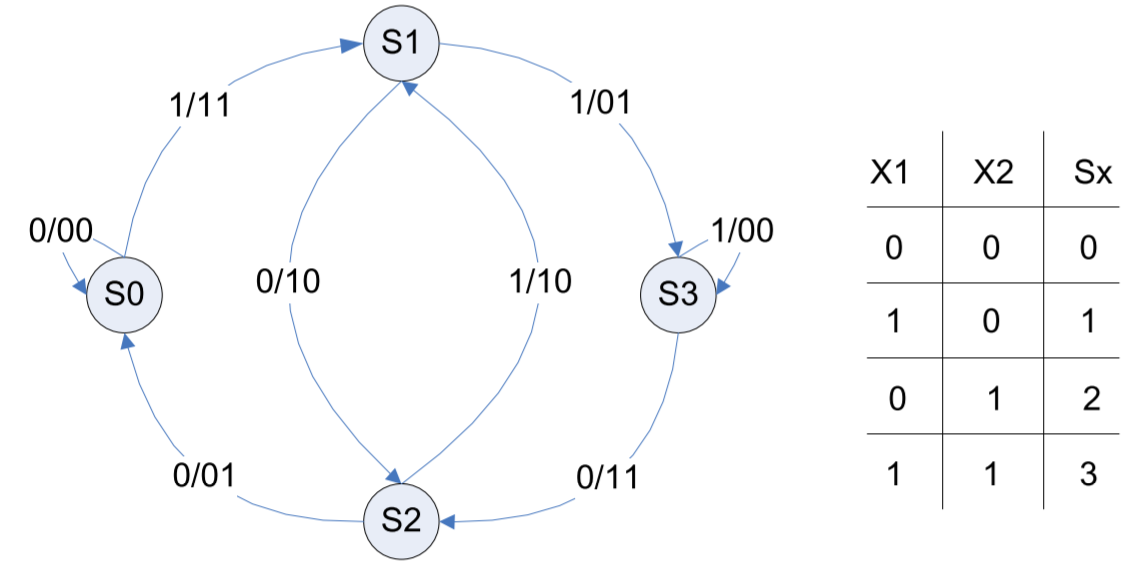
\includegraphics[width=.8\linewidth]{./02-kanalcodierung/fs2009_8}
    \vspace{-8pt}
\end{center}

Lieft ein katastrophaler Code vor?\\
\textit{Ja, da keine Gewichtszunahme beim Zustand S3 wenn eine 1 kommt. 1 Folge geht in eine 0 Folge über.}\\

Ermitteln Sie für die Nachrichtenfolge {u[n]}={1,1,1,0,1,1} die Ausgangscodefolge {v[n]}.\\
${v[n]}={1,1,0,1,0,0,1,1,1,0,0,1,Tailbits,1,1,0,1}$\\

Bestimmen sie für das obige Beispiel die (Block-)Coderate.\\
$R=b/n$\\
$b=Eingabebits=6$\\
$n=Ausgabebits=6*2+2*2 (Tail-Bits)$\\
$R=6/16=0.375$

\subsection{Kanalmatrix}
\subsubsection{Prüfung HS2016}
Die Eigenschaften eines Kanals seien durch die folgende Kanalmatrix beschrieben: 

$P(Y|X) = \begin{matrix}
    0.4 & 0.5 & 0.1\\
    0.3 & 0.4 & 0.3\\
    0.3 & 0.1 & 0.6
\end{matrix}$

\paragraph{Bestimmen Sie die Entscheidungszuordnung nach dem Maximum Likelyhood-Verfahren:}\mbox{}\\
$P(Y|X) = \begin{matrix}
    \textcolor{red}{0.4} & \textcolor{red}{0.5} & 0.1\\
    0.3 & 0.4 & 0.3\\
    0.3 & 0.1 & \textcolor{red}{0.6}
\end{matrix}$

\paragraph{}\mbox{Maximum Likelihood}\\
Berechnen Sie die Restfehlerwahrscheinlichkeit für die nach dem Maximum Li-kelyhood-Verfahren gefundene Entscheidungszuordnung\\
Gehen Sie davon aus, dass alle Eingangszeichen gleichwahrscheinlich auftreten.\\

$p(restfehler) = 1 - [1/3*(0.4+0.5+0.6)] = 0.5$\\

In einer vertieften Analyse der Eingangszeichen wurden folgende Auftrittshäufigkeiten festge-stellt:\\
$x1 = 500$\\
$x2 = 2500$\\
$x3 = 7000$\\

Lässt sich mit dieser zusätzlichen Information eine Entscheidungszuordnung finden, die besser ist als die nach dem Maximum Likelyhood-Verfahren gefunde-ne? Begründen Sie Ihren Entscheid.
$p(x1) = 0.05$\\
$p(x2) = 0.25$\\
$p(x3) = 0.70$\\


$P(Y|X) = \begin{matrix}
    \textcolor{red}{0.4} & 0.5 & 0.1\\
    0.3 & \textcolor{red}{0.4} & 0.3\\
    0.3 & 0.1 & \textcolor{red}{0.6}
\end{matrix}$

$p(rest) = 1-(0.05*0.4 + 0.25*0.4 + 0.7*0.6) = 0.46 $\\

ist kleiner als 0.5 und auch kleiner als wenn Restfehlerwahrscheinlichkeit mit der Analyse für 	die ursprünglich gewählte Konfiguration:\\
$1 - (0.05*0.4 + 0.05*0.5 + 0.7*0.6) = 0.535$

\subsection{Kanal}
\subsubsection{Prüfung FS2015}
Messungen an einem symmetrischen Kanal, ergeben die unten angegebenen Auftrittswahrscheinlichkeiten der Zeichen am Kanaleingang respektive am Kanalausgang.\\
\begin{center}
    \vspace{-8pt}
    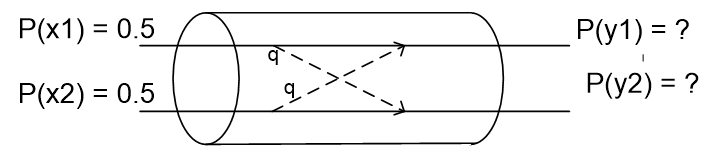
\includegraphics[width=.8\linewidth]{./02-kanalcodierung/fs2015}
    \vspace{-8pt}
\end{center}

Die Kanalmatrix ist gegeben mit:

$P(X|Y) = \begin{matrix}
    0.9 & 0.1\\
    0.2 & 0.8\\
\end{matrix}$

Ermitteln sie die Entropie am Kanaleingang H(x) und am Kanalausgang H(y). Ist der Kanal fehlerfrei?\\
$p(y_1)=0.5*0.9+0.5*0.2=0.55$\\
$p(y_2)=0.5*0.1+0.5*0.8=0.45$\\

$H(X)=-\sum_{i=1}^3p(x_i)*ld(p(x_i))$\\
$=-(0.5*ld(0.5)+0.5*ld(0.5))$\\
$=1$\\

$H(Y)=-\sum_{i=1}^3p(y_i)*ld(p(y_i))$\\
$=-(0.55*ld(0.55)+0.45*ld(0.45))$\\
$=0.99$\\

Der Kanal ist nicht fehlerfrei!

\subsection{Transinformation}
\subsubsection{Prüfung FS2009}
Sie messen einen binären Kanal aus und erhalten folgende Ergebnisse:\\

\begin{center}
    \centering
    \begin{tabular}{l | l | l}
        \bfseries{Zeichen} & \bfseries{gesendet}& \bfseries{Korrekt Empfangen}\\ \hline
        1 & 1000 & 980\\ 
        0 & 1000 & 650
    \end{tabular}
\end{center}

\paragraph{Geben Sie die Kanalmatrix an}\mbox{}\\

$\begin{bmatrix}
    0.98 & 0.02\\
    0.35 & 0.65\\
\end{bmatrix}$

Sie haben ebenfalls herausgefunden, dass die Auftrittswahrscheinlichkeiten der 2 Zeichen wie folgt ist:
\begin{itemize}
    \item Auftrittswahrscheinlichkeit für eine 1: P(1) = 0.7
    \item Auftrittswahrscheinlichkeit für eine 0: P(0) = 0.3
\end{itemize}

\paragraph{Berechnen Sie die Entropie für den Kanaleingang und den Kanalausgang}\mbox{}\\
$y_0=0.7*0.98+0.3*0.35=0.791$\\
$y_1=0.7*0.02+0.3*0.65=0.209$\\

$H(X)=-\sum_{i=1}^mp(x_i)*ld(p(x_i))$\\
Eingang: $H(X)=-(0.7*ld(0.7)+0.3*ld(0.3))=0.8813$\\
Ausgang: $H(Y)=-(0.791*ld(0.791)+0.209*ld(0.209))=0.7395$

\paragraph{Wie gross ist die Transinformation}\mbox{}\\
\begin{center}
    \vspace{-8pt}
    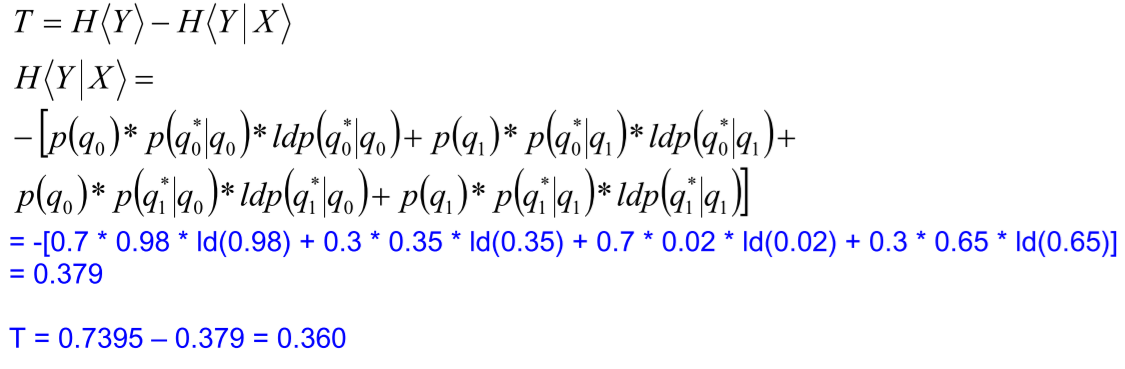
\includegraphics[width=.8\linewidth]{./02-kanalcodierung/fs2009}
    \vspace{-8pt}
\end{center}




        %! Licence = CC BY-NC-SA 4.0

%! Author = gianfluetsch
%! Date = 22. Jan 2022
%! Project = icth_summary

\section{Signale}
\subsection{Rinkel}
\subsubsection{FS2015}
Sie planen einen Subwoofer zu bauen und wissen, dass die minimale Phasenverschie-bung zwischen dem linken und rechten Ohr, die ein Mensch zur Lokalisierung der Schallquelle noch auswerten kann bei 0.2 rad liegt.
Bestimmen sie die obere Grenzfrequenz, die der Subwoofer maximal abgeben darf.\\

Gehen sie dabei von den folgenden Annahmen aus. Der Abstand von einem Ohr zum anderen ist  im Mittel mit 21 cm gegeben. Die Schallgeschwindigkeit wird mit 330 m/s angenommen.\\

Stellen sie die maximale Phasenverschiebung des Audiosignals von einem zum anderen Ohr als Funktion der Frequenz dar.\\

$\phi(f)=2\pi f s/v = f = \frac{\phi}{2\pi}*\frac{s}{v}$\\
$f=\frac{0.2*330 m/s}{2\pi*0.21m} = 50 Hz$\\

Fourier:  Gegeben ist ein Generator der folgendes Dreieckssignal mit der Frequenz von 3 kHz generiert:
\begin{center}
    \vspace{-8pt}
    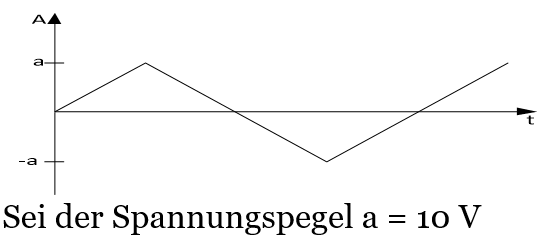
\includegraphics[width=.6\linewidth]{./03-signale/fs2015}
    \vspace{-8pt}
\end{center}

Sie wollen ein harmonisches Signal mit der Frequenz von 9 kHz erzeugen. Entwickeln Sie eine Prinzipschaltung unter Angabe aller signifikanten Werte, die dies realisiert.\\
$y(t)=\frac{8\hat{y}}{\pi^2}(\frac{1}{1^2}*sin(\omega_0 t)-\frac{1}{3^2}*sin(3\omega_0 t)+\frac{1}{5^2}*sin(5\omega_0 t)-...)$\\
\textit{Die Frequenz von 9 kHz entspricht der zweiten harmonischen $\rightarrow$ durch einen Bandpass mit der unteren Grezfrequenz von z.B. 8 khz und einer oberen Grenzfrequenz von z. Bsp 10 kHz }\\

Wie gross ist die Amplitude dieser harmonischen Schwingung?\\
$a=\frac{8*10V}{9*\pi^2}=0.9V$\\

Um wie viel db ist dann das Ausgangssignal gegenüber dem Eingangssignal gedämpft?\\
$a=10log\frac{0.9V}{10V}=-10.46db$\\

Wie hoch ist dann der Pegel in V beim Empfänger, wenn die nachgeschaltete Übertra-gungsstrecke eine Dämpfung von 3 db aufweist?\\
$-13.46db = 10log\frac{x}{10}$\\
$10^{-1.346}*10V = 0.045V$

\subsubsection{Prüfung HS2009}
Zur Verschleierung von Sprachsignalen wird das System in Bild unten, auch Scrambler genannt, eingesetzt. Es transformiert das Signalspektrum in die Kehrlage und wurde beispielweise im Mobilfunknetz C eingesetzt.\\
\begin{center}
    \vspace{-8pt}
    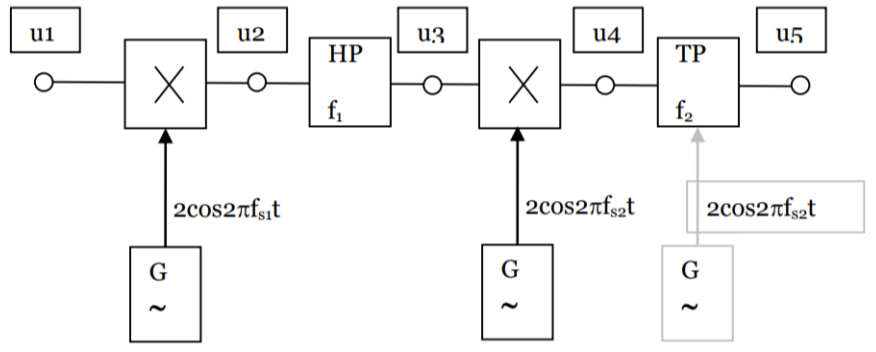
\includegraphics[width=.6\linewidth]{./03-signale/hs2009_6}
    \vspace{-8pt}
\end{center}

Was versteht man unter Kehrlage eines Signals?\\
\textit{Das höherfrequente Nachchtensignal liegt in beiden Seitenbändern näher bei der Trägerfrequenz als das niedfrequente Nachrichtensignal.}\\

Analysieren Sie das System, indem Sie die Spektren der Signale u1 bis u5 skizzieren. Es ist g die Grenzfrequenz des Eingangssignals u1.\\
Geben Sie ferner die Frequenzen f1, f2 sowie fs1 und fs2 zueinander so an, dass der Scrambler seine Aufgabe erfüllen kann.
\begin{center}
    \vspace{-8pt}
    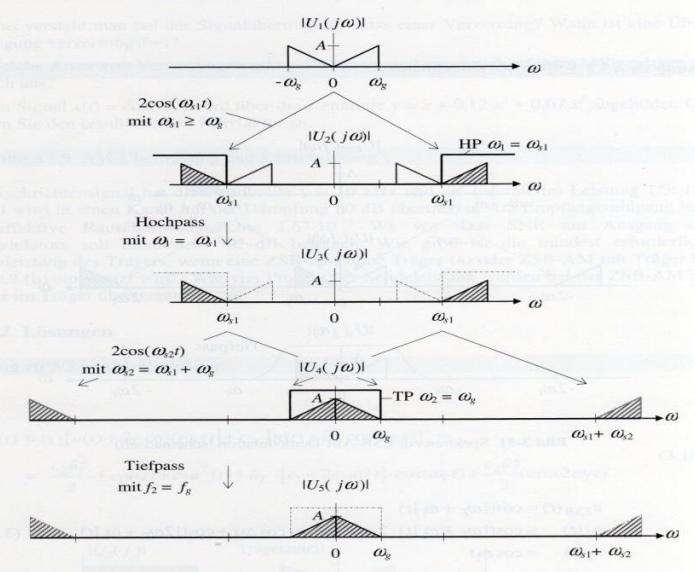
\includegraphics[width=.6\linewidth]{./03-signale/hs2009_7}
    \vspace{-8pt}
\end{center}

Gegeben ist das folgende Spektrum eines modulierten Sprachsignals.
\begin{center}
    \vspace{-8pt}
    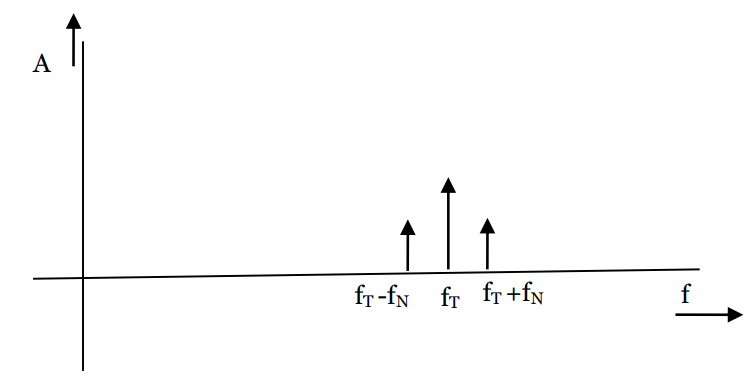
\includegraphics[width=.6\linewidth]{./03-signale/hs2009_8}
    \vspace{-8pt}
\end{center}

Befindet sich das Sprachsignal fN in der Kehr- oder Regellage? (Anm. die Frequenz fN ist die obere Grenzfrequenz des Sprachsignals)\\
\textit{Das Signal befindet sich nicht in der Kehrlage.}\\

Konstruieren Sie eine Demodulatoschaltung und zeigen sie rechnerisch, dass das Sprachsignal fN im Basisband vorliegt.\\
\begin{center}
    \vspace{-8pt}
    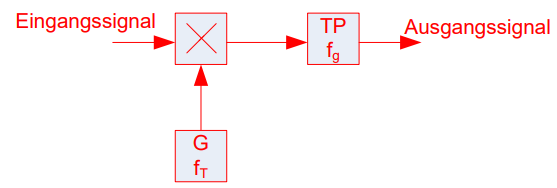
\includegraphics[width=.6\linewidth]{./03-signale/hs2009_9}
    \vspace{-8pt}
\end{center}

\begin{center}
    \vspace{-8pt}
    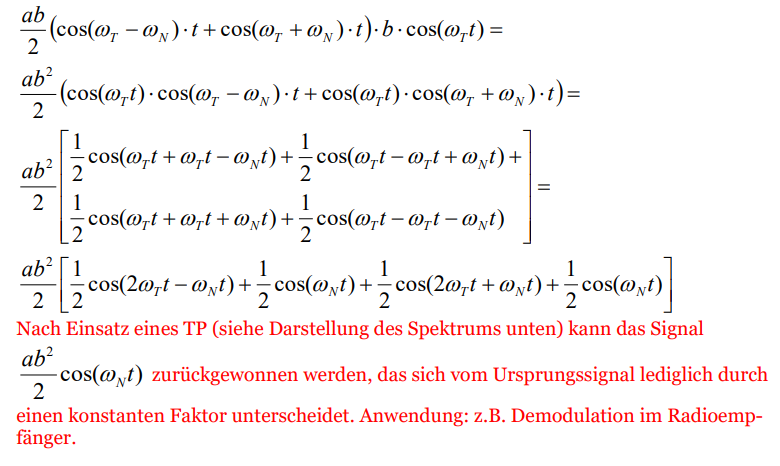
\includegraphics[width=.8\linewidth]{./03-signale/hs2009_10}
    \vspace{-8pt}
\end{center}

\subsubsection{Prüfung FS2009}
Gegeben ist das folgende Blockschaltbild:
\begin{center}
    \vspace{-8pt}
    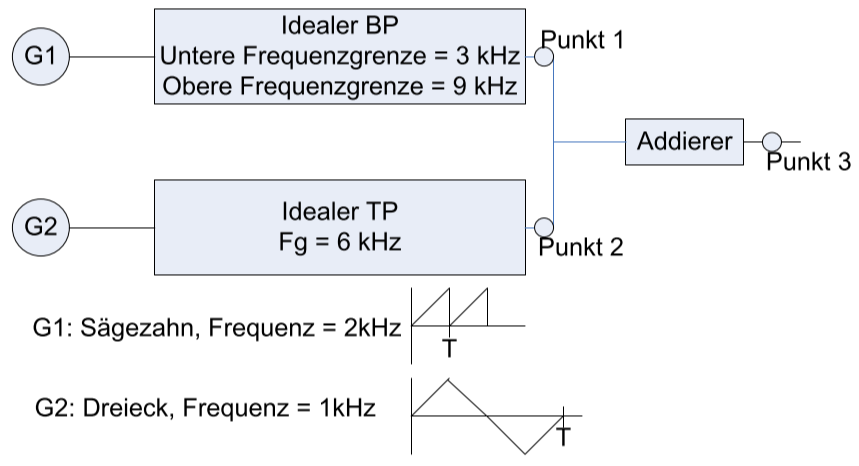
\includegraphics[width=.8\linewidth]{./03-signale/fs2009}
    \vspace{-8pt}
\end{center}

Zeichnen Sie das Frequenzspektrum, das Sie an dem Punkt1, dem Punkt 2 und dem Punkt 3 beobachten können.\\
\textit{Die Fourierzerlegung folgt für}\\
$f(x)=a(sin(x)+\frac{sin(2x)}{2}+\frac{sin(3x)}{3}+...)$\\

\textit{Das positive Sägezahnsignal zu:}\\
$f(x)=a(\frac{1}{1^2}*sin(x)-\frac{sin(3x)}{3^2}+\frac{sin(5x)}{5^2}-....)$\\

\textit{Und das Dreieckssignal zu:}
\begin{center}
    \vspace{-8pt}
    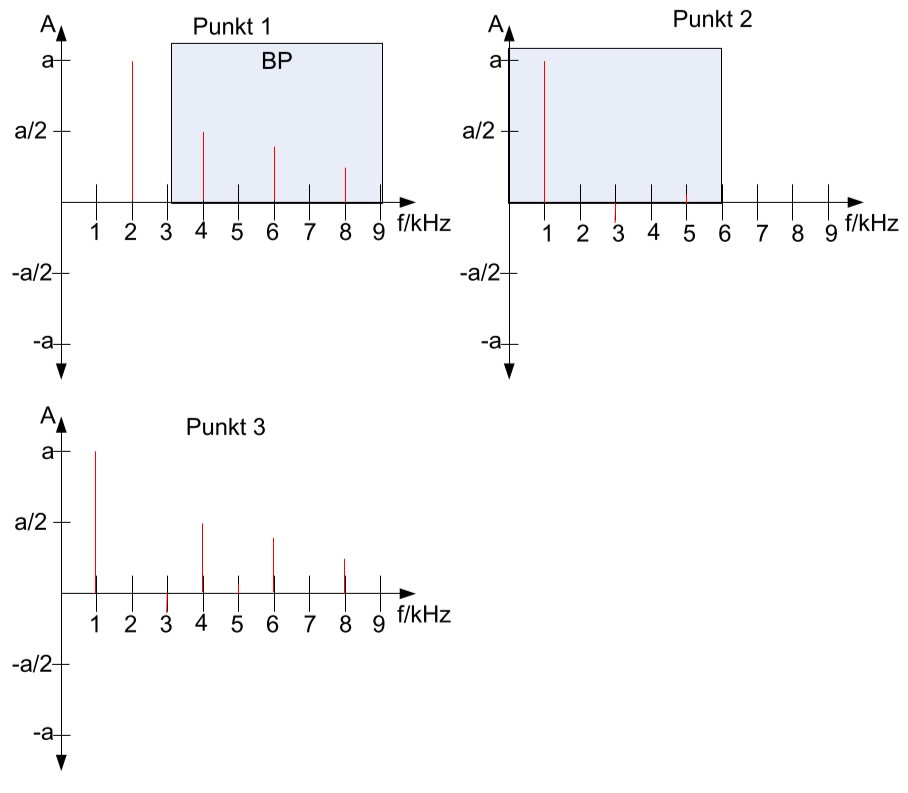
\includegraphics[width=.8\linewidth]{./03-signale/fs2009_2}
    \vspace{-8pt}
\end{center}




        %! Licence = CC BY-NC-SA 4.0

%! Author = gianfluetsch
%! Date = 22. Jan 2022
%! Project = icth_summary

\section{Quantisierung}
\subsection{Rinkel}
\subsubsection{Prüfung FS2009}
\textbf{Ist es nach einer Quantisierung möglich das originale Analoge Signal zu 100\% wieder herzustellen? (Mit Begründung).}\\
Nein, das analoge Signal wird aus dem digitalen Signal lediglich rekonstriert. Es ist jedoch von geringerer Qualität als das Originalsignal. Diese Differenz zwischen den Signalen wird durch
den Quantisierungsfehler hervorgerufen.\\

\textbf{Welche Grund-Bitrate wird für ein Sprachsignal (digitale Übertragung der Sprache in einem Telefonkanal) benötigt? (Berechnung und Begründung)}\\
Die Sprache hat einen Umfang von0,3-3,4 kHz. Nach inernationalen Normen wird ein Frequenzspektrum von 4kHz angenommen. Daraus folgt die Abtastfrequenz 2*4kHz = 8kHz. Im weiteren sind $2^12$ Quantisierungsstufen zu wählen. Durch die Kompandierung werden diese vor der Übertragung auf 8 bit komprimiert. Dies ergibt eine CW-Länge von 8Bit. Die
Bitrate folgt nun aus der Abtastfrequenz und der CW-Bitlänge 8kHz * 8 Bit = 64kBit/s
        %! Licence = CC BY-NC-SA 4.0

%! Author = gianfluetsch
%! Date = 22. Jan 2022
%! Project = icth_summary

\section{Leitungscodierung}
\subsection{Rinkel}
\subsubsection{Prüfung FS2009}
Ein NRZ Signal hat den unten aufgezeichneten Signalverlauf. Skizzieren Sie den entsprechenden Signalverlauf sowohl für den Manchester Code als auch für den AMI-Code.
\begin{center}
    \vspace{-8pt}
    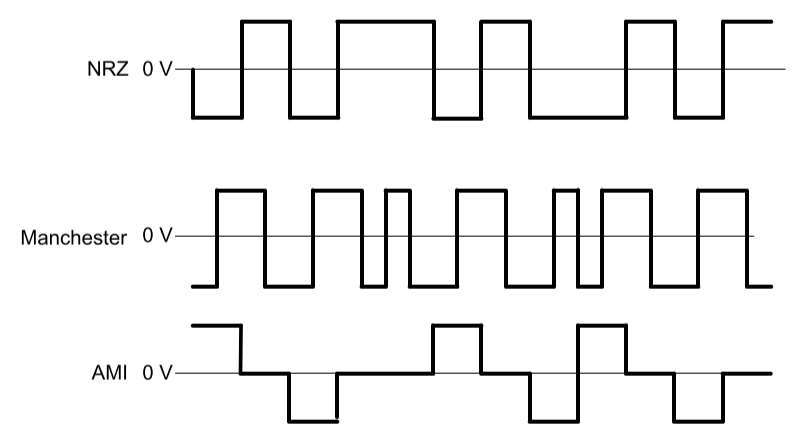
\includegraphics[width=.8\linewidth]{./06-leitungscodierung/fs2009}
    \vspace{-8pt}
\end{center}

\textbf{Vergleichen Sie die drei Codierungsarten anhand der oben gegebenen und der erstellten Codierungen.}\\
Lange 0-Folgen werden beim AMI Code zu einem Problem wegen der Phasen und Taktrückgewinnung. NRZ hat dieselben Probleme der Phasen- und Taktrückgewinnung bei
langen 0 oder 1 Folgen. Der Manchestercode weist bei jedem Bit einen Pegelwechsel auf.

\subsection{Steffen}

\subsubsection{Nachprüfung HS2020}
In der untentstehenden Grafik wird ein binäres Datensignal mittels einer Leitungscodes über einen Kommunikationskanal übertragen:
\begin{center}
    \vspace{-8pt}
    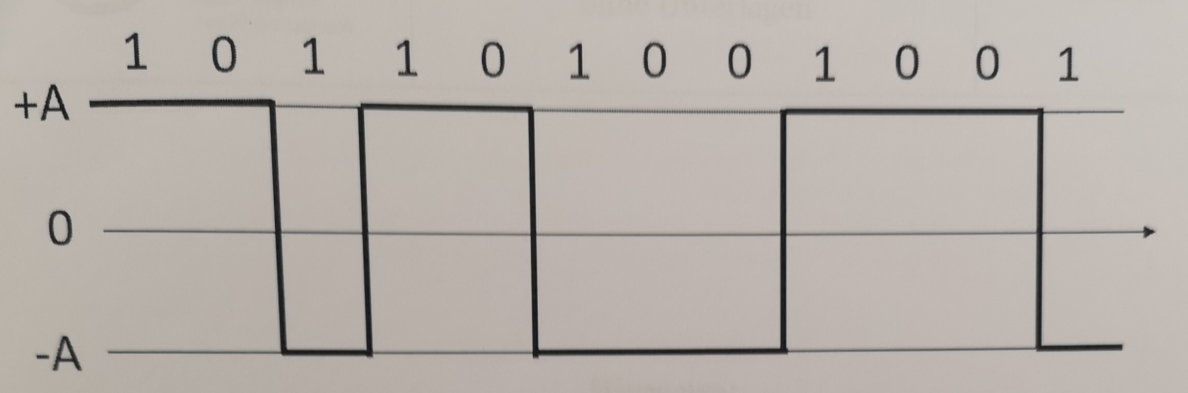
\includegraphics[width=.9\linewidth]{./06-leitungscodierung/hs2020-2}
    \vspace{-8pt}
\end{center}

\textbf{Um welchen Leitungscode handelt es sich?}\\
Bipolarer NRZ (Non Return to Zero) Code.\\

\textbf{Ist der Leitungscode bei allen möglichen Datensequenzen mittelwertfrei?}\\
$\rightarrow$ nicht mittelwertfrei, da lange '0'-Folgen entweder einen positiven oder negativen DC-Offset bewirken.\\

\textbf{Bei welchen Datensequenzen könnte beim Empfänger der Takt verloren gehen?}\\
Der Takt kann bei langen '0'-Folgen verloren gehen, da keine Pegelwechsel stattfinden.\\

\textbf{Mit welcher Zusatzmassnahme könnte die Mittelwertfreiheit und die Taktextraktion mit hoher Wahrscheinlichkeit garantiert werden?}\\
Durch Scramkeln der Datensequenz vor der Leitungscodierung könnte die Mittelwertfreiheit und die Taktextraktion mit hoher Wahrscheinlichkeit garantiert werden.

\subsubsection{Prüfung HS2018}
Eine Datenquelle sendet dauernd die Nullsequenz $'... 0 0 0 0 0 0 ...'$. Kreuzen Sie an, ob die unten aufgeführten Leitungscodes für diese Sequenz annähernd gleichspannungsfrei sind, respektive ob genügend Pegelwechsel für eine Taktrückgewinnung vorhanden sind.
\begin{center}
    \vspace{-8pt}
    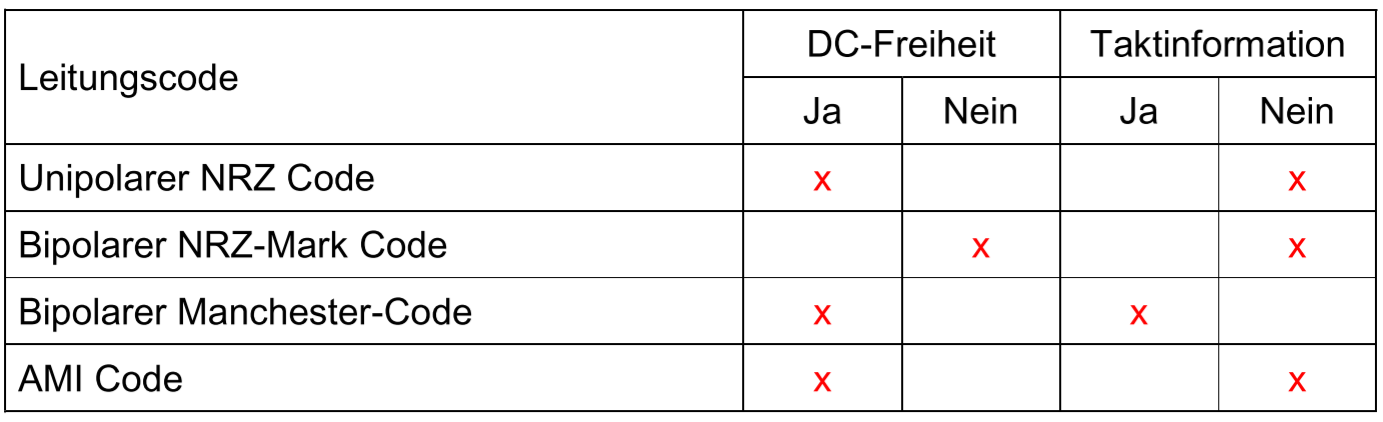
\includegraphics[width=.9\linewidth]{./06-leitungscodierung/hs2018}
    \vspace{-8pt}
\end{center}

\subsubsection{Prüfung HS2016}
Eine Datenquelle sendet dauernd die Einersequenz $'....1 1 1 1 1 1 ...'$. Kreuzen Sie an, ob die unten aufgeführten Leitungscodes für diese Sequenz annähernd gleichspannungsfrei sind, res-
pektive ob genügend Pegelwechsel für eine Taktrückgewinnung vorhanden sind.
\begin{center}
    \vspace{-8pt}
    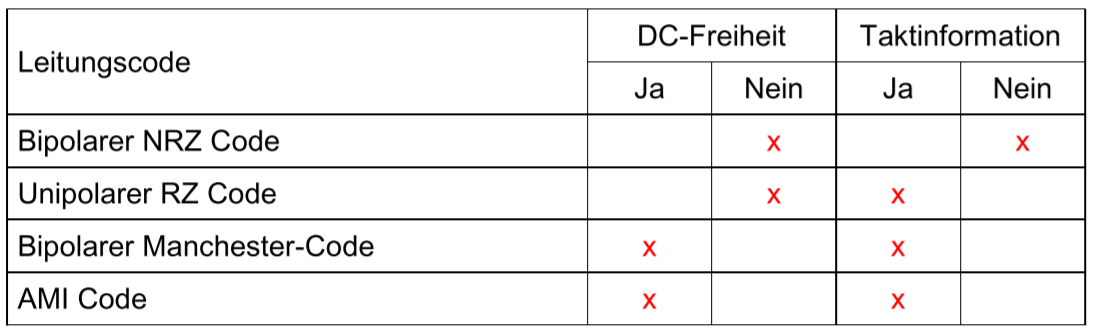
\includegraphics[width=.9\linewidth]{./06-leitungscodierung/hs2016}
    \vspace{-8pt}
\end{center}

        %! Licence = CC BY-NC-SA 4.0

%! Author = gianfluetsch
%! Date = 22. Jan 2022
%! Project = icth_summary

\section{Quadrature Amplitude Modulation (QAM)}

\subsubsection{Nachprüfung HS2020}
Ein binärer Datenstrom soll via eine 64-QAM Modulation über ein verdrilltes Kupferaderpaar übertragen werden.\\
In der unterstehenden Signalebene sind die Signalpunkte eingetragen.Wie gross ist der Abstand jedes Signalpunktes von der nächsten Entscheidungsschwelle?\\
\begin{center}
    \vspace{-8pt}
    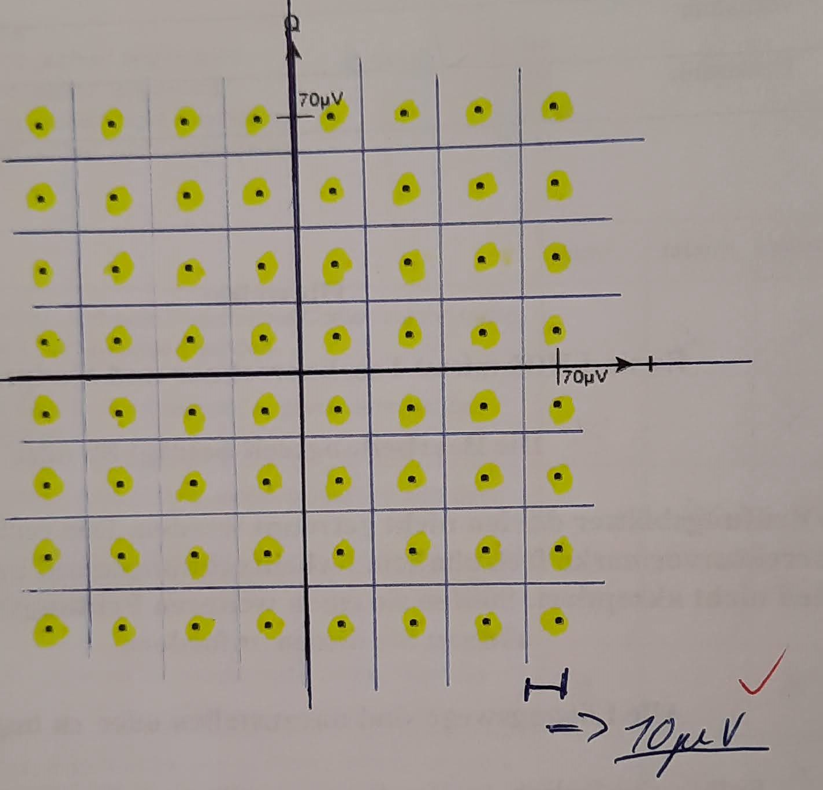
\includegraphics[width=.5\linewidth]{./07-qam/hs2020-2}
    \vspace{-8pt}
\end{center}

\textbf{Wie gross wird bei $U_{eff}=1\mu V$ (entspricht einer Bitfehlerrate $BER = 10^{-23}$) die mittlere Rauschleistung N in [W] an einem Widerstand von $R=100\Omega$? 
Drücken Sie diese Rauschleistung auch als N in [dBm] aus.}\\
$N=\frac{(U_{eff})^2}{R}=\frac{(1'-{-6})^2}{100\Omega} \rightarrow 10^{-4}W=0.01pW$\\
$10*log_{10}(\frac{10^{-14}}{10^{-3}})=10*log(10^{-11})=-110dBm$

\subsubsection{Prüfung HS2019}
Ein binärer Datenstrom soll via eine 64-QAM Modulation über ein verdrilltes Kupferaderpaar mit Wellenimpedanz $Zw = 100 \Omega $  übertragen werden.\\
In der unterstehenden komplexen Signalebene sind die vier Signalpunkte mit der grössten Leistung eingetragen. Ergänzen Sie das 64-QAM Modulationsschema und zeichnen Sie
die Entscheidungsschwellen ein.\\
\begin{center}
    \vspace{-8pt}
    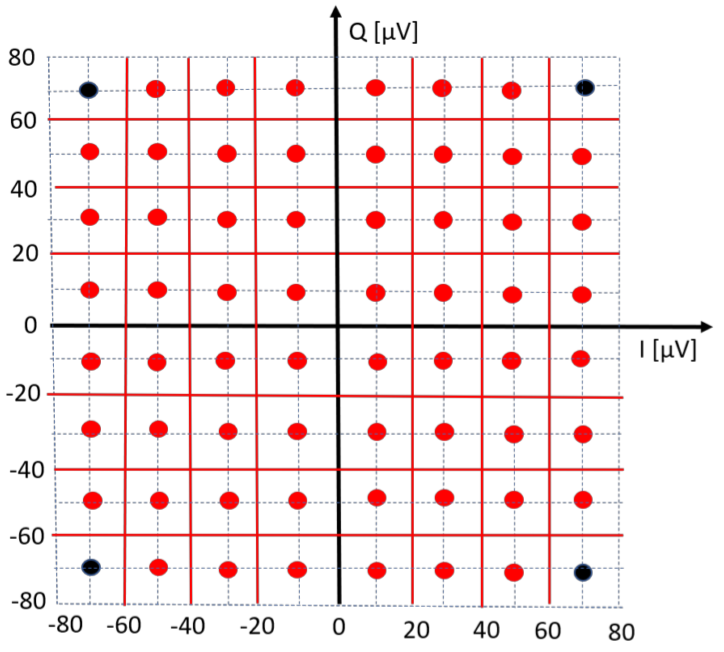
\includegraphics[width=.5\linewidth]{./07-qam/hs2019}
    \vspace{-8pt}
\end{center}

\textbf{Wie gross ist der Abstand jedes Signalpunkts von der nächsten Entscheidungsschwelle?}\\
$50\mu V$\\

\textbf{Welchen Effektivwert $U_{eff}$ darf das normalverteilte Rauschen haben, wenn das Signal-zu-Rauschverhältnis \textbf{SNR = 20 dB} sein soll, damit eine Bitfehlerrate \textit{$BER = 10^{-23}$} resultiert?}\\
$1\mu V$\\

\textbf{Wie gross wird beim oben bestimmten Ueff die mittlere Rauschleistung N in [W] an einem Widerstand von $R = 100 \Omega$? Drücken Sie diese Rauschleistung auch als N in [dBm] aus.}\\
$N=\frac{U_{eff}^2}{R}=\frac{(10^{-6})^2}{100}=10^{-14}W=0.01pW$\\
$N=10log_{10}\frac{N}{10^{-3}}=10log(10-{-11})=-110dBm$\\

\textbf{Da es sich um weisses Rauschen handelt, gilt $N=10logkT\Delta f=-174dBm+10log\Delta f$.
Wie gross darf die Systembandbreite B maximal sein, damit der oben berechnete Rauschpegel für die 64-QAM Detektion nicht überschritten wird?}\\
$10logB=N+174dBm=-110dBm+174dBm=64dB$\\
$\rightarrow$ Systembandbreite: $B=10Mhz/4=2.5MHz$\\

\textbf{Wie hoch darf die Bitrate des mit 64-QAM modulierten Datenstroms maximal sein, damit die Bitfehlerrate \textbf{$BER = 10^{-23}$} eingehalten wird?}\\
Da mit 64-QAM 6 Bit pro Symbol übertragen werden können, resultiert eine Bitrate von 15 Mbit/s.\\
Weil B=2.5MHz $\rightarrow$ Symbolrate max 2.5MBaud, da 64 QAM (also 6 Bit pro Symbol) $\rightarrow$ Bitrate von 15Mbits/s (2.5 MBaud*6Bit).\\
Wegen der vorgegebenen Systembandbreite von B = 2.5 MHz darf die Symbolrate maximal 2.5 MBaud sein.


        %! Licence = CC BY-NC-SA 4.0

%! Author = gianfluetsch
%! Date = 22. Jan 2022
%! Project = icth_summary

\section{Dauer und Bandbreite von Einzelpulsen}

\subsubsection{A}
Ein parabelförmiger Puls s(t) hat folgenden zeitlichen Verlauf:
\begin{center}
    \vspace{-8pt}
    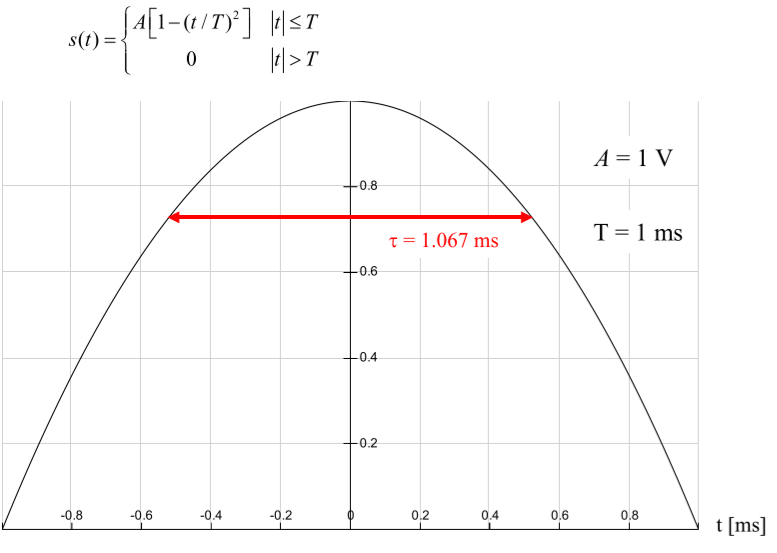
\includegraphics[width=.8\linewidth]{./08-einzelpulse/hs2019}
    \vspace{-8pt}
\end{center}

Das zweiseitige Amplitudendichtespektrum S(f) in [V/Hz] berechnet sich aus dem zeitkontinuierlichen Signal s(t) über die Fouriertransformation zu
\begin{center}
    \vspace{-8pt}
    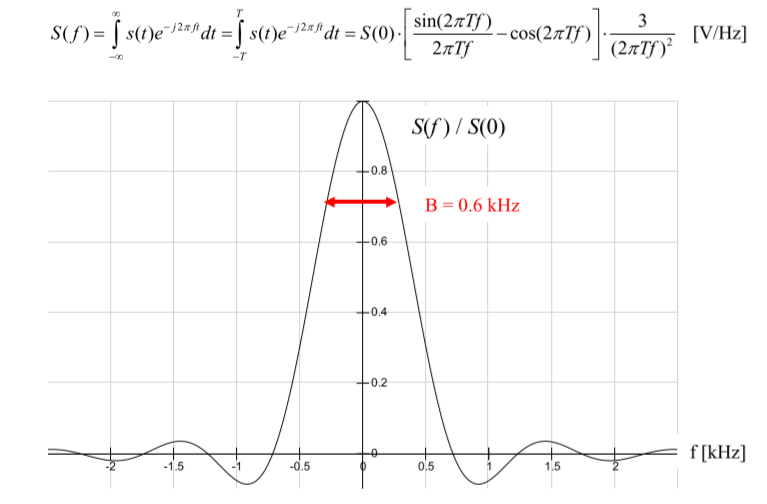
\includegraphics[width=.8\linewidth]{./08-einzelpulse/hs2019_1}
    \vspace{-8pt}
\end{center}

\textbf{Wie ist das asymptotische Verhalten des Amplitudendichtespektrums S(f) für |f | >> 1?}\\
Quadratische Abnahme mit $1/f^2$\\

\textbf{Wie kann S(0), d.h. die Amplitudendichte bei der Frequenz f = 0 Hz aus dem Verlauf des parabelförmigen Pulses s(t) berechnet werden? Benützen Sie als Hilfe die analytische
Lösung des folgenden Integrals:}\\
$\int_{-T}^{T} (1-\frac{t^2}{T^2})dt=\frac{4}{3}T$\\

\textbf{Geben Sie die Formel für S(0), sowie den numerischen Wert in [V/Hz] an}\\
Für f=0 gilt: $S(0)=\int_{-\infty}^{\infty}s(t)dt=\int_{-T}^{T}A(1-\frac{t^2}{T^2})dt=\frac{4}{3}AT$\\
Der numerische Wert ist: S(0) = 4/3 V * 1ms = 1.33 mV/Hz\\

\textbf{Die im parabelförmigen Puls s(t) enthaltene Energie kann mit folgender Formel berechnet werden}\\
$E=\int_{-\infty}^{\infty}p(t)dt=\int_{-\infty}^{\infty}\frac{s^2(t)}{R}dt=\frac{1}{R}\int_{-T}^{T}s^2(t)dt=\frac{16}{15}\frac{A^2T}{R} [Ws]$\\

\textbf{Wie gross ist die Energie E in [J] oder [Ws] an einem Widerstand $R = 1 \Omega$?}\\
$E = 16/15 * 1 V^2 * 1ms / 1 \Omega = 16/15 mWs = 1.067 mJ$\\

\textbf{Wie gross ist die Dauer $\tau$ eines äquivalenten Rechteckpulses $r(t)$ mit Amplitude A und dem gleichen Energieinhalt an $R = 1 \Omega$ wie der parabelförmige Puls s(t)? Leiten Sie die Formel for die äquivalente Rechteckdauer $\tau $ als Formel her und bestimmen Sie den numerischen Wert in [s].}\\
$A=\frac{A^2\tau}{R}=\frac{16}{15}\frac{A^2T}{R}$\\
$\tau = \frac{16}{15}T$ und damit $\tau =16/15 ms = 1.067ms$\\

\textbf{Wie gross ist die Bandbreite B eines äquivalenten rechteckförmigen Spektrums mit gleicher Amplitudedichte S(0) und gleichem Energieinhalt an $R = 1 \Omega$ wie das Amplitudendichtespektrum S(f) des parabelförmigen Pulses s(t)? Leiten Sie die Formel für die äquivalente Rechteckbandbreite B als Formel her und bestimmen Sie den numerischen Wert in [Hz].}\\
$E=\frac{|S(0)|^2B}{R}=\frac{16}{9}\frac{A^2T^2B}{R}=\frac{16}{15}\frac{A^2T}{R}$\\
$B=\frac{3}{5}\frac{1}{T}$ und damit $B=3/5 kHz=0.6kHz$\\

\textbf{Wie gross ist das Zeit-Bandbreiteprodukt $B_{\tau }$ des parabelförmigen Pulses s(t)?}\\
$B_{\tau }=\frac{3}{5}\frac{1}{T}*\frac{16}{15}T=\frac{16}{25}=0.64$

\subsubsection{B}
Der sogenannte \textit{Raised-Cosine} Einzelpuls s(t) hat folgenden zeitlichen Verlauf:
\begin{center}
    \vspace{-8pt}
    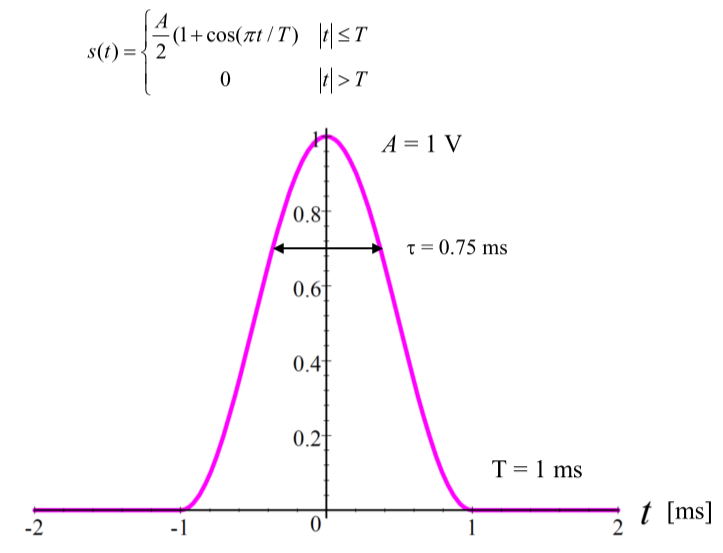
\includegraphics[width=.8\linewidth]{./08-einzelpulse/hs2018}
    \vspace{-8pt}
\end{center}

Das zweiseitige Amplitudendichtespektrum S(f) in [V/Hz] berechnet sich aus dem zeitkontinuierlichen Signal s(t) über die Fouriertransformation zu
\begin{center}
    \vspace{-8pt}
    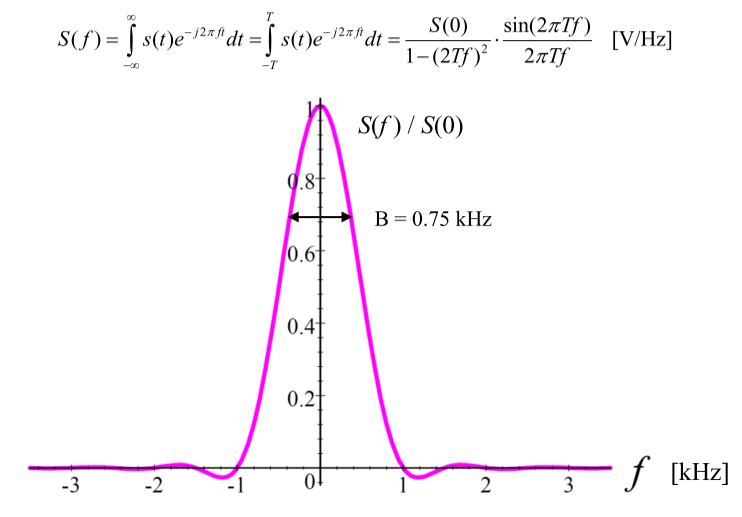
\includegraphics[width=.8\linewidth]{./08-einzelpulse/hs2018_1}
    \vspace{-8pt}
\end{center}

\textbf{Wie kann S(0), d.h. die Amplitudendichte bei der Frequenz $f=0 Hz$, einfach aus dem Verlauf des Raised-Cosine Pulses s(t) berechnet werden? Geben Sie die Formel für S(0),}
sowie den numerischen Wert in [V/Hz] an.\\
Für f = 0 gilt: $S(0)=\int_{-\infty}^{\infty}s(t)dt=\int_{-T}^{T}s(t)dt=AT$\\
d.h. die Gesamtfläche A/2*2T unter dem Gleichspannungswert, da die Fläche des Cosinus über eine Periode gerade Null ergibt.\\
Der nummerische Wert ist: $S(0)=1V*1ms=1mv/Hz$\\

\textbf{Die im \textit{Raised-Cosine} Pulse s(t) enthaltene Energie kann mit folgender Formel berechnet werden}\\
$E=\int_{-\infty}^{\infty}p(t)dt=\int_{-\infty}^{\infty}\frac{s^2(t)}{R}dt=\frac{1}{R}\int_{-T}^{T}s^2(t)dt=\frac{3}{4}\frac{A^2T}{R}[Ws]$\\

\textbf{Wie gross ist die Energie E in [J] oder [Ws] an einem Widerstand $R = 1 \Omega$?}\\
$E = 3/4 * 1 V^2 * 1ms / 1 \Omega  = 3/4 mWs = 0.75 mJ$\\

\textbf{Wie gross ist die Dauer $\tau $ eines äquivalenten Rechteckpulses r(t) mit Amplitude A und dem gleichen Energieinhalt an $R = 1 \Omega$ wie der Raised-Cosine Puls s(t)? Leiten Sie die Formel for die äquivalente Rechteckdauer $\tau $als Formel her und bestimmen Sie den numerischen Wert in [s].}\\
$E=\frac{A^2 \tau }{R}=\frac{3}{4}\frac{A^2T}{R}$\\
$\tau=\frac{3}{4}T \rightarrow \tau=3/4 ms = 0.75ms$\\

\textbf{Wie gross ist die Bandbreite B eines äquivalenten rechteckförmigen Spektrums mit gleicher Amplitudedichte S(0) und gleichem Energieinhalt an $R = 1 \Omega$ wie das Amplitudendichtespektrum S(f) des Raised-Cosine Pulses s(t)? Leiten Sie die Formel für die äquivalente Rechteckbandbreite B als Formel her und bestimmen Sie den numerischen Wert in [Hz].}\\
$R=1\Omega$\\
$E=\frac{|S(0)|^2*B}{R}=\frac{A^2T^2B}{R}=\frac{3}{4}\frac{A^2T}{R}$\\
$B=\frac{3}{4}\frac{1}{T} \rightarrow \tau = 3/4 kHz = 0.75 kHz$\\

\textbf{Wie gross ist das Zeit-Bandbreiteprodukt $B_{\tau}$ des Raised-Cosine Pulses s(t)?}\\
$B_{\tau}=\frac{3}{4}*\frac{1}{T}*\frac{3}{4}T=\frac{9}{16}=0.5625$

\subsubsection{C}
Ein dreieckförmiger Einzelpuls s(t) hat folgenden zeitlichen Verlauf:
\begin{center}
    \vspace{-8pt}
    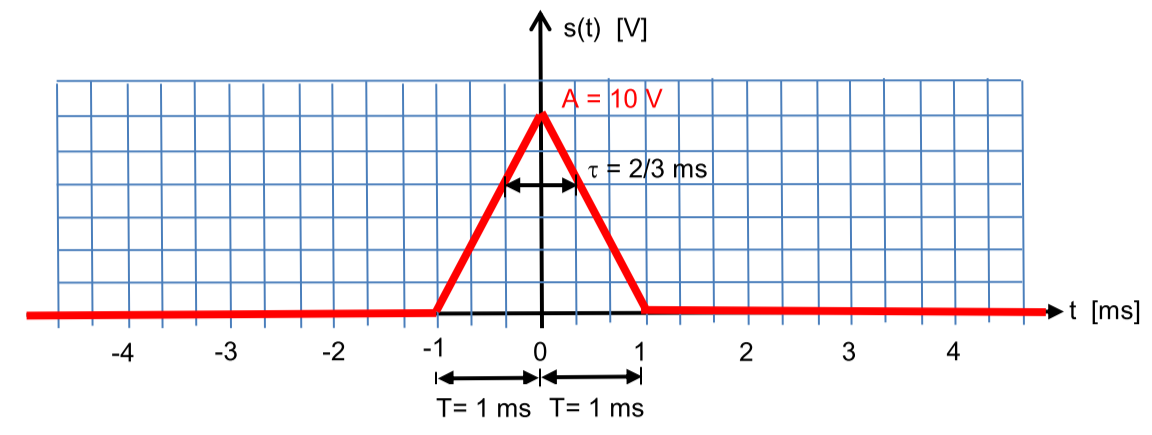
\includegraphics[width=.5\linewidth]{./08-einzelpulse/hs2017}
    \vspace{-8pt}
\end{center}

Das zweiseitige Amplitudendichtespektrum S(f) in [V/Hz] berechnet sich aus dem zeitkontinuierlichen Signal s(t) über die Fouriertransformation zu\\
\begin{center}
    \vspace{-8pt}
    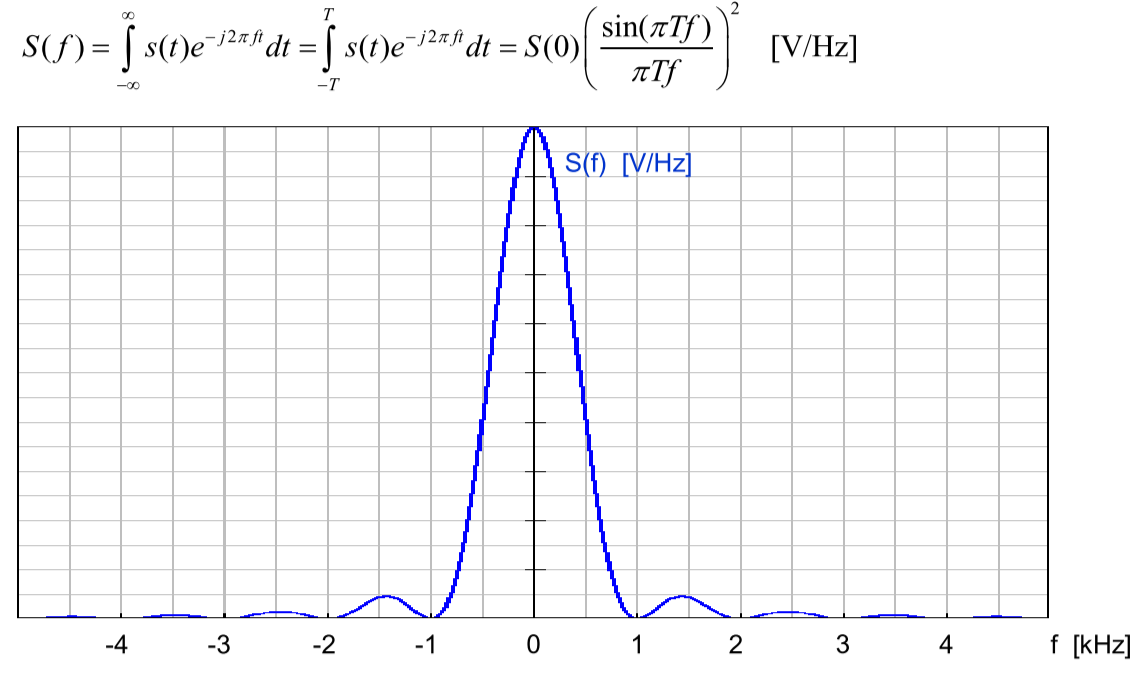
\includegraphics[width=.5\linewidth]{./08-einzelpulse/hs2017_2}
    \vspace{-8pt}
\end{center}

\textbf{Wie kann S(0), d.h. die Amplitudendichte bei der Frequenz f = 0 Hz, \textbf{einfach} aus dem Verlauf des Dreieckpulses s(t) berechnet werden? Geben Sie die Formel für S(0), sowie
den numerischen Wert in [V/Hz] an.}\\
Für f=0 gilt: $S(0)=\int_{-\infty}^{\infty}s(t)dt=\int_{-T}^{T}s(t)dt=AT$\\

d.h. die Gesamtfläche unter der Dreiecksfunktion s(t).\\
Der numerische Wert ist: $S(0)=10V*1ms=10mv/Hz$\\

\textbf{Die im Dreieckspuls s(t) enthaltene Energie kann mit folgender Formel berechnet werden}\\
$E=\int_{-\infty}^{\infty}p(t)dt=\int_{-\infty}^{\infty}\frac{s^2(t)}{R}dt=\frac{1}{R}\int_{-T}^{T}s^2(t)dt=\frac{3}{4}\frac{A^2T}{R}[Ws]$\\

\textbf{Wie gross ist die Energie E in [J] oder [Ws] an einem Widerstand $R = 50 \Omega$?}\\
$E = 2/3 * 100 V^2 * 1ms / 50 \Omega = 4/3 mWs = 1.333 mJ$

\textbf{Wie gross ist die Dauer $\tau$ eines äquivalenten Rechteckpulses r(t) mit Amplitude A und dem gleichen Energieinhalt an $R = 50 \Omega$ wie der Dreieckpuls s(t)? Leiten Sie die Formel for die äquivalente Rechteckdauer $\tau$ als Formel her und bestimmen Sie den numerischen
Wert in [s].}\\
$E=\frac{A^2 \tau }{R}=\frac{3}{4}\frac{A^2T}{R}$\\
$\tau=\frac{3}{4}T$ und damit $\tau=3/4 ms = 0.75ms$\\

\textbf{Wie gross ist die Bandbreite B eines äquivalenten rechteckförmigen Spektrums mit gleicher Amplitudedichte S(0) und gleichem Energieinhalt an $R = 50 \Omega$ wie das Amplitudendichtespektrum S(f) des Raised-Cosine Pulses s(t)? Leiten Sie die Formel für die äquivalente Rechteckbandbreite B als Formel her und bestimmen Sie den numerischen Wert in [Hz].}\\
$E=\frac{|S(0)|^2B}{R}=\frac{A^2T^2B}{R}=\frac{2}{3}\frac{A^2T}{R}$\\
$B=\frac{2}{3}\frac{1}{T}$ und damit $\tau = 2/3 kHz = 0.666 kHz$\\

\textbf{Wie gross ist das Zeit-Bandbreiteprodukt $B_{\tau}$ des Dreieckpulses s(t)?}\\
$B_{\tau}=\frac{2}{3}\frac{1}{T}*\frac{2}{3}T=\frac{4}{9}=0.444$
        %! Licence = CC BY-NC-SA 4.0

%! Author = gianfluetsch
%! Date = 22. Jan 2022
%! Project = icth_summary

\section{Abtastung von BPSK-Signalen}

\subsubsection{Prüfung HS2019}
Ein zufälliges bipolares NRZ Datensignal d(t) mit einer Datenrate von 2 Mbit/s wird mit Binary Phase Shift Keying (BPSK) auf eineTrägerfrequenz $f_0 = 5 MHz$ aufmoduliert:\\
$s(t)=d(t)cos(2\pi f_0t)$\\

Das modulierte Trägersignal s(t) hat folgendes zweiseitiges Dichtespektrum S(f):\\
\begin{center}
    \vspace{-8pt}
    \includegraphics[width=.5\linewidth]{./08-einzelpulse/hs2019_2}
    \vspace{-8pt}
\end{center}

Dieses Trägersignal s(t) wird nun mit einer Samplingfrequenz $f_s = 5 MHz$ abgetastet. Zeichnen Sie das resultierende zweiseitige Spektrum des abgetasteten Signals in die
untenstehende Grafik ein:
\begin{center}
    \vspace{-8pt}
    \includegraphics[width=.5\linewidth]{./08-einzelpulse/hs2019_3}
    \vspace{-8pt}
\end{center}

Tritt bei dieser Abtastung Aliasing auf? Begründen Sie Ihre Antwort.\\
\textit{Nein es tritt kein Aliasing auf, da sich die periodischen Spektrumswiederholungen nicht überlappen und damit wieder herausgefiltert werden können}.\\

Was bewirkt die gezielte Wahl der Sampling Frequenz $f_s = f_0$?\\
\textit{Das Sampling mit der Trägerfrequenz $f_0$ bewirkt ein Verschiebung des Datensignals in das Basisband und damit eine Produktdemodulation mit $f_0$}.\\

In der folgenden Grafik ist das BPSK-modulierte Trägersignal s(t) dargestellt. Tragen Sie darin die Abtastwerte s[n] ein, die wie folgt definiert sind:\\
$s[n]=s(n*\delta t)$ mit $\delta t = \frac{1}{f_s}$
\begin{center}
    \vspace{-8pt}
    \includegraphics[width=.5\linewidth]{./09-bpsk/hs2019_4}
    \vspace{-8pt}
\end{center}

Was stellt das zeitkontinuierliche Signal dar, welches durch Interpolation aus den Abtastwerten s[n] rekonstruiert werden kann?\\
\textit{Das rekonstruierte Signal stellt angenähert das bipolare NRZ Datensignal d(t) dar.}\\

Welche Datenbits werden durch den obenstehenden Ausschnitt der BPSK Modulation übertragen, unter der Annahme, dass $0°$ Phase eine logische Eins und $180°$ eine logische
Null codiert?\\
\textit{Die Datenfolge lautet: 0 1 1 0 1 0}

\subsubsection{Prüfung HS2018}
Ein zufälliges bipolares NRZ Datensignal d(t) mit einer Datenrate von 2 Mbit/s wird mit Binary Phase Shift Keying (BPSK) auf eineTrägerfrequenz $f_0 = 5 MHz$ aufmoduliert:\\
$s(t)=d(t)cos(2\pi f_0t)$\\
Das modulierte Trägersignal s(t) hat folgendes zweiseitiges Dichtespektrum S(f):
\begin{center}
    \vspace{-8pt}
    \includegraphics[width=.5\linewidth]{./09-bpsk/hs2018}
    \vspace{-8pt}
\end{center}

Dieses Trägersignal s(t) wird nun mit einer Samplingfrequenz $f_s = 5 MHz$ abgetastet. Zeichnen Sie das resultierende zweiseitige Spektrum des abgetasteten Signals in die
untenstehende Grafik ein:
\begin{center}
    \vspace{-8pt}
    \includegraphics[width=.5\linewidth]{./09-bpsk/hs2018_2}
    \vspace{-8pt}
\end{center}

Tritt bei dieser Abtastung Aliasing auf? Begründen Sie Ihre Antwort.\\
\textit{Nein es tritt kein Aliasing auf, da sich die periodischen Spektrumswiederholungen nicht überlappen und damit wieder herausgefiltert werden können.}\\

Was bewirkt die gezielte Wahl der Sampling Frequenz $f_s = f_0$?\\
\textit{Das Sampling mit der Trägerfrequenz $f_0$ bewirkt ein Verschiebung des Datensignals in das Basisband und damit eine Produktdemodulation mit $f_0$.}\\

In der folgenden Grafik ist das BPSK-modulierte Trägersignal s(t) dargestellt. Tragen Sie darin die Abtastwerte s[n] ein, die wie folgt definiert sind:\\
$s[n]=s(n*\delta t)$ mit $\delta t=\frac{1}{f_s}$
\begin{center}
    \vspace{-8pt}
    \includegraphics[width=.5\linewidth]{./09-bpsk/hs2018_3}
    \vspace{-8pt}
\end{center}

Was stellt das zeitkontinuierliche Signal dar, welches durch Interpolation aus den Abtastwerten s[n] rekonstruiert werden kann?\\
\textit{Das rekonstruierte Signal stellt angenähert (1 P) das bipolare NRZ Datensignal d(t) dar.}\\

Welche Datenbits werden durch den obenstehenden Ausschnitt der BPSK Modulation übertragen, unter der Annahme, dass 0° Phase eine logische Eins und 180° eine logische
Null codiert?\\
\textit{Die Datenfolge lautet: 1 0 1 1 0 1}



        %! Licence = CC BY-NC-SA 4.0

%! Author = gianfluetsch
%! Date = 22. Jan 2022
%! Project = icth_summary

\section{Produktmodulation}

\subsubsection{A}
Ein auf einen Träger von 20 MHz aufmoduliertes Datensignal soll mittels Produktmodulation auf eine Sendefrequenz von 100 MHz verschoben werden.\\
\begin{itemize}
    \item Mit welchen zwei Modulatorfrequenzen (Lösung 1 und 2) kann dies erreicht werden?
    \item Zeichnen Sie das zweiseitige Spektrum nach der Produktmodulation in die zwei untenstehenden Grafiken ein.
    \item Welche Filter werden in Lösung 1, respektive 2 benötigt, damit nur das Datensignal bei 100 MHz ausgesendet wird?
\end{itemize}

\begin{center}
    \vspace{-8pt}
    \includegraphics[width=.9\linewidth]{./10-produktmanipulation/hs2019_5}
    \vspace{-8pt}
\end{center}
        %! Licence = CC BY-NC-SA 4.0

%! Author = gianfluetsch
%! Date = 22. Jan 2022
%! Project = icth_summary

\section{Signal-to-Noise Ration und Pegelplan}

\subsubsection{Prüfung HS2018}
Ein drahtgebundenes Übertragungssystem hat eine Systembandbreite B = 2 GHz.\\

Wie gross ist die thermische Rauschleistung [in dBm] in dieser Systembandbreite? Bitte Herleitung angeben, nicht nur numerisches Endresultat.\\
$N=-174dBm+10logB=-174dBm+10log(2*10^9)$\\
$N=-174dBm + 3 dB + 90 dB = -81dBm$\\

Der Empfänger in diesem Übertragungssystem besteht aus einem Bandpassfilter mit 2 GHz Bandbreite und 2 dB Einfügungsdämpfung und einem nachgeschalteten Mischer
mit 8 dB Einfügungsdämpfung. Es sollen folgende Randbedingungen gelten:
\begin{itemize}
    \item Der Signal-zu-Rauschabstand (SNR) an jeder Stelle des Pegelplans soll mindestens +20 dB betragen, damit eine geringe Bitfehlerrate garantiert ist.
    \item Der maximale Signalpegel am Eingang des Mischers darf maximal +5 dBm betragen, damit nicht zu viele ungewollte Mischprodukte entstehen.
\end{itemize}

Tragen Sie diese beiden Randbedingungen in den untenstehenden Pegelplan ein und bestimmen Sie anschliessend grafisch im Pegelplan den Verlauf für den minimalen und
maximalen Pegel:
\begin{center}
    \vspace{-8pt}
    \includegraphics[width=.6\linewidth]{./11-pegelplan/hs2018}
    \vspace{-8pt}
\end{center}

Wie gross werden gemäss des obenstehenden Pegelplans der maximale und minimale Pegel [in dBm] am Eingang des Empfängers und welche Signaldynamik [in dB] resultiert?\\
$S_{max}=+7dBm$\\
$S_{min}=-51dBm$\\

$Signaldynamik = S_{max}-S_{min}=+7dBm+51dBm=58dB$

\subsubsection{Prüfung HS2017}
Ein drahtloses Übertragungssystem hat eine Systembandbreite B = 80 MHz.\\

Wie gross ist die thermische Rauschleistung [in dBm] in dieser Systembandbreite? Bitte Herleitung angeben, nicht nur numerisches Endresultat.\\
$N=-174dBm+10logB=-174dBm+10log(2*2*2*10^7)$\\
$N=-174dBm + 3 dB + 3 dB + 3 dB + 70 dB = -95dBm$\\

Der Empfänger in diesem drahtlosen Übertragungssystem besteht aus einem Bandpassfilter mit 80 MHz Bandbreite und 3 dB Einfügungsdämpfung und einem nachgeschalteten
Verstärker mit 30 dB Verstärkung. Es sollen folgende Randbedingungen gelten:
\begin{itemize}
    \item Der Signal-zu-Rauschabstand (SNR) an jeder Stelle des Pegelplans soll mindestens +15 dB betragen, damit eine geringe Bitfehlerrate garantiert ist.
    \item Der maximale Signalpegel am Ausgang des Verstärkers soll maximal +10 dBm betragen, damit keine Signalverzerrungen auftreten
\end{itemize}
Tragen Sie diese beiden Randbedingungen in den untenstehenden Pegelplan ein und bestimmen Sie anschliessend grafisch im Pegelplan den Verlauf für den minimalen und
maximalen Pegel:
\begin{center}
    \vspace{-8pt}
    \includegraphics[width=.6\linewidth]{./11-pegelplan/hs2017}
    \vspace{-8pt}
\end{center}

Wie gross werden gemäss des obenstehenden Pegelplans der maximale und minimale Pegel [in dBm] am Eingang des Empfängers und welche Signaldynamik [in dB] resultiert?\\
$S_{max}=-17dBm$\\
$S_{min}=-77dBm$\\

$Signaldynamik = S_{max}-S_{min}=-17dBm+77dBm=60dB$

        %! Licence = CC BY-NC-SA 4.0

%! Author = gianfluetsch
%! Date = 22. Jan 2022
%! Project = icth_summary

\section{Digitale Modulationsarten}

\subsubsection{A}
Die Datensequenz $'1 1 1 0 0 0 0 1 0 1 0 1'$ wird bei einer festen Bitrate von 1 MBit/s mittels vier verschiedener Modulationsarten übertragen. Charakterisieren Sie die verwendeten Verfahren und stellen Sie jeweils die Wertigkeit M der Symbole, d.h. die Anzahl übertragener
Bits pro Symbol fest!
\begin{center}
    \vspace{-8pt}
    \includegraphics[width=.8\linewidth]{./12-modulationsarten/hs2017}
    \vspace{-8pt}
\end{center}
\begin{center}
    \vspace{-8pt}
    \includegraphics[width=.8\linewidth]{./12-modulationsarten/hs2017_1}
    \vspace{-8pt}
\end{center}

\subsubsection{B}
Bauen sie einen Modulator. Führen Sie dazu die Multiplikation der beiden Signalen $S_N = acos(\omega_Nt)$ und $S_T = bcos(\omega_Tt)$ durch. Betrachten sie das resultierende Signal im Zeit- und Frequenzbereich. Wählen sie für das Modell  die konkreten Grössen $f_T = 3500Hz$ und $fN = 1000...5000Hz$ aus, die Amplituden a und b jeweils 1...10V.\\

\textbf{Interpretieren Sie das Ergebnis mathematisch bezüglich der spektralen Eigenschaften des neuen Signals unter der Annahme, dass $S_N$ ein niederfrequentes Nachrichtensignal und $S_T$ ein hochfrequentes Trägersignal ist.}\\
$S_T*S_N=abcos(\omega_Tt)cos(\omega_Nt)$\\
$=\frac{ab}{2}(cos((\omega_T-\omega_N)t)+cos((\omega_T+\omega_N)t))$\\
Durch die Multiplikation der beiden Signale wird das niederfrequente Signal um die Frequenz des sogenannten Trägersignals (um die Werte $\omega_T -\omega_N$ und $\omega_T+\omega_N$) verschoben oder transponiert. Somit kann das ursprüngliche Signal in einen Frequenzbereich gebracht werden, der sich für eine Abstrahlung eignet (zum Beispiel für eine Radio Amplitudenmodulation in KW, MW oder LW):
\begin{center}
    \vspace{-8pt}
    \includegraphics[width=.8\linewidth]{./12-modulationsarten/w11}
    \vspace{-8pt}
\end{center}

Ergänzen Sie einen De-Modulator. Führen Sie dazu wieder die Multiplikation des modulierten Signals mit dem Trägersignal $ST = bcos(\omega_Tt+\varphi )$ durch.
Machen sie beim Demodulationssignal Amplitude, Frequenz und Phase variabel.\\
$S_T*(S_T*S_N)=\frac{ab^2}{2}cos(\omega_Tt)(cos((\omega_T-\omega_N)t)+cos((\omega_T+\omega_N)t))$\\
$=\frac{ab^2}{4}cos((\omega_Tt+\omega_T-\omega_N)t)+cos((\omega_T-\omega_T+\omega_N)t))$\\
$+\frac{ab^2}{4}cos((\omega_Tt+\omega_T+\omega_N)t)+cos((\omega_T-\omega_T-\omega_N)t))$\\
$=\frac{ab^2}{4}cos((2\omega_Tt-\omega_N)t)+cos((2\omega_T+\omega_N)t))$\\
$+\frac{ab^2}{4}(cos(\omega_Nt)+cos(-\omega_Nt))$\\
$=\frac{ab^2}{4}(cos((2\omega_T-\omega_N)t)+cos((2\omega_T+\omega_N)t))+\frac{ab^2}{2}cos(\omega_Nt)$\\

Durch die erneute Multiplikation werden die bereits modulierten Signale nochmals um die Trägerfrequenz $S_T$ verschoben (um die Werte $\omega_T-(\omega_T\pm \omega_N)$ und $\omega_T+(\omega_N\pm  \omega_T)$):
\begin{center}
    \vspace{-8pt}
    \includegraphics[width=.8\linewidth]{./12-modulationsarten/w11_2}
    \vspace{-8pt}
\end{center}

Mit Berücksichtigung der Phase gilt:\\
$S_T*(S_T*S_N)=\frac{ab^2}{2}cos(\omega_Tt+\varphi )(cos((\omega_T-\omega_N)t)+cos((\omega_T+\omega_N)t))$\\
$=\frac{ab^2}{4}cos((\omega_Tt+\omega_T-\omega_N)t+\varphi )+cos((\omega_T-\omega_T+\omega_N)t+\varphi ))$\\
$+\frac{ab^2}{4}cos((\omega_Tt+\omega_T+\omega_N)t+\varphi )+cos((\omega_T-\omega_T-\omega_N)t+\varphi ))$\\
$=\frac{ab^2}{4}cos((2\omega_T-\omega_N)t+\varphi )+cos((2\omega_T+\omega_N)t+\varphi ))$\\
$+\frac{ab^2}{4}(cos(\varphi +\omega_Nt)+cos(\varphi -\omega_Nt))$\\
$=\frac{ab^2}{4}cos(\varphi )(cos((2\omega_T+\omega_N)t)+\frac{ab^2}{2}cos(\varphi )cos(\omega_Nt)$\\
D.h. ist $\varphi $ ein ungerades Vielfaches von $\frac{\pi}{2}$, so kommt es zur Signalauslöschung.\\

\textbf{Was braucht es, damit die Demodulation fehlerfrei funktioniert?}\\
Damit die Demodulation fehlerfrei funktioniert, braucht es einen Tiefpassfilter, welcher das obere Seitenband der Demodulation herausfiltert. Zudem muss das Demodulationssignal die gleiche Trägerfrequenz und Phasenlage haben.\\

\textbf{Gegeben ist die folgende Prinzipschaltung:}
\begin{center}
    \vspace{-8pt}
    \includegraphics[width=.8\linewidth]{./12-modulationsarten/w11_3}
    \vspace{-8pt}
\end{center}

Hierbei sei $\omega_N$ das Nutzdatensignal und $\omega_T$ das Trägersignal.\\

\textbf{Ermitteln Sie das Frequenzspektrum des Signale mathematisch am Referenzpunkt 1.}\\
$S_1=1+cos(\omega_Nt)+cos(\omega_Tt)$\\

\textbf{Ermitteln Sie das Frequenzspektrum des Signale mit DasyLab und mathematisch am Referenzpunkt 2.}\\
$S_2=S_1^2=(1+cos(\omega_Nt)+cos(\omega_Tt))^2$\\
$=1+cos^2(\omega_Nt)+cos^2(\omega_Tt)+2cos(\omega_Nt)+2cos(\omega_Tt)+2cos(\omega_Nt)cos(\omega_Tt)$\\
$=1+\frac{1}{2}cos(2\omega_Nt)+\frac{1}{2}cos(0)+\frac{1}{2}cos(2\omega_Tt)+\frac{1}{2}cos(0)$\\
$+2cos(\omega_Nt)+2cos(\omega_Tt)+cos((\omega_T+\omega_N)t)+cos((\omega_T-\omega_N)t)$\\
$=2+\frac{1}{2}cos(2\omega_Nt)+\frac{1}{2}cos(2\omega_Tt)$\\
$+2cos(\omega_Nt)+2cos(\omega_Tt)+cos((\omega_T+\omega_N)t)+cos((\omega_T-\omega_N)t)$\\

\textbf{Bestimmen Sie System X so, das am Ausgang ein amplitudenmoduliertes Signal mit Träger anliegt.}\\
Ein Bandpass mit einer unteren Grenzfrequenz von $\omega_T-\omega_N$ und einer oberen Grenzfrequenz von $\omega_T+\omega_N$.
        %! Licence = CC BY-NC-SA 4.0

%! Author = gianfluetsch
%! Date = 22. Jan 2022
%! Project = icth_summary

\section{Audiosignalen}

\subsection{Tonhöhenverschiebung von Audiosignalen}
\subsubsection{A}
Ein Audiosignal s(t) hat folgendes zweiseitiges Dichtespektrum S(f):

\begin{center}
    \vspace{-8pt}
    \includegraphics[width=.6\linewidth]{./13-audiosignale/hs2017}
    \vspace{-8pt}
\end{center}

Dieses Audiosignal s(t) wird nun mit einem Produktmodulator auf eine Trägerfrequenz von 8 kHz verschoben, so dass das untenstehende Spektrum resultiert:
\begin{center}
    \vspace{-8pt}
    \includegraphics[width=.6\linewidth]{./13-audiosignale/hs2017_2}
    \vspace{-8pt}
\end{center}

Beschreiben Sie im Detail zwei Lösungen, die es erlauben, die Tonhöhe des Audiosignals um 200 Hz anzuheben (Mickey Mouse), so dass das untenstehende Ausgangsspektrum resultiert.
\begin{center}
    \vspace{-8pt}
    \includegraphics[width=.6\linewidth]{./13-audiosignale/hs2017_3}
    \vspace{-8pt}
\end{center}

\paragraph{Lösung 1}\mbox{}\\
\begin{itemize}
    \item Elimination des oberen Seitenbandes (USB) durch ein Tiefpassfilter mit der Grenzfrequenz 8 kHz
    \item Demodulation mit einer LO-Frequenz von 8200 Hz, welches das untere Seitenband (LSB) mit einem Frequenzshift von +200 Hz in das Basisband zurückschiebt
\end{itemize}

\paragraph{Lösung 2}\mbox{}\\
\begin{itemize}
    \item Elimination des unteren Seitenbandes (LSB) durch ein Hochpassfilter mit der Grenzfrequenz 8 kHz
    \item Demodulation mit einer LO-Frequenz von 7800 Hz, welches das obere Seitenband (USB) mit einem Frequenzshift von 1200 Hz in das Basisband zurückschiebt
\end{itemize}

\paragraph{Lösung 3}\mbox{}\\
\begin{itemize}
    \item Durch die Demodulation entsteht eine Spektrumskomponente bei der doppelten Trägerfrequenz von ca. 16 kHz
    \item Diese hörbaren Frequenzanteile können mit einem Tiefpassfilter eliminiert werden
\end{itemize}

\subsection{Abtastung von Audiosignalen}
\subsubsection{A}
Ein nichtperiodisches Audiosignal s(t) hat folgendes zweiseitiges Dichtespektrum S(f):
\begin{center}
    \vspace{-8pt}
    \includegraphics[width=.6\linewidth]{./13-audiosignale/hs2016}
    \vspace{-8pt}
\end{center}

Dieses Audiosignal s(t) wird nun mit einer Samplingfrequenz $f_s = 10 kHz$ abgetastet. Zeichnen Sie das resultierende zweiseitige Spektrum des abgetasteten Audiosignals in die
untenstehende Grafik ein:
\begin{center}
    \vspace{-8pt}
    \includegraphics[width=.6\linewidth]{./13-audiosignale/hs2016_2}
    \vspace{-8pt}
\end{center}

\textbf{Tritt bei der Abtastfrequenz von $f_s = 10 kHz$ Aliasing auf?}\\
Nein es tritt kein Aliasing auf, da die höchste im Audiosignal vorkommende Frequenz von 4 kHz kleiner als die Hälfte der Abtastfrequenz $f_s/2 = 5 kHz$ ist und sich deshalb die periodischen Spektrumswiederholungen nicht überlappen.\\

Als Alternative wird das Audiosignal s(t) mit einer tieferen Samplingfrequenz $f_s = 7 kHz$ abgetastet. Zeichnen Sie das resultiererende zweiseitige Spektrum des abgetasteten Audio-
signals in die untenstehende Grafik ein:
\begin{center}
    \vspace{-8pt}
    \includegraphics[width=.6\linewidth]{./13-audiosignale/hs2016_3}
    \vspace{-8pt}
\end{center}

\textbf{Tritt bei der Abtastfrequenz von $f_s = 7 kHz$ Aliasing auf?}\\
Ja es tritt Aliasing auf, da die höchste im Audiosignal vorkommende Frequenz von 4 kHz grösser als die Hälfte der Abtastfrequenz $f_s/2 = 3.5 kHz$ ist und sich deshalb die
periodischen Spektrumswiederholungen überlappen.\\

\textbf{Wie kann bei einer gegebenen Abtastfrequenz $f_s$ das Auftreten von Aliasing beim Abtasten vermieden werden?}\\
Durch Vorschalten eines Tiefpassfilters mit einer Grenzfrequenz $f_g < f_s/2$, so dass keine Spektrumsüberlappungen auftreten.

    \end{multicols*}

\end{document}
